%%%%%%%%%%%%%%%%%%%%%%%%%%%%%%%%%%%%%%%%%
% Beamer Presentation
% LaTeX Template
% Version 1.0 (10/11/12)
%
% This template has been downloaded from:
% http://www.LaTeXTemplates.com
%
% License:
% CC BY-NC-SA 3.0 (http://creativecommons.org/licenses/by-nc-sa/3.0/)
%
%%%%%%%%%%%%%%%%%%%%%%%%%%%%%%%%%%%%%%%%%

%----------------------------------------------------------------------------------------
%saPACKAGES AND THEMES
%----------------------------------------------------------------------------------------

\documentclass{beamer}

\mode<presentation> {

% The Beamer class comes with a number of default slide themes
% which change the colors and layouts of slides. Below this is a list
% of all the themes, uncomment each in turn to see what they look like.

%\usetheme{default}
%\usetheme{AnnArbor}
%\usetheme{Antibes}
%\usetheme{Bergen}
%\usetheme{Berkeley}
%\usetheme{Berlin}
%\usetheme{Boadilla}
%\usetheme{CambridgeUS}
%\usetheme{Copenhagen}
%\usetheme{Darmstadt}
%\usetheme{Dresden}
%\usetheme{Frankfurt}
%\usetheme{Goettingen}
%\usetheme{Hannover}
%\usetheme{Ilmenau}
%\usetheme{JuanLesPins}
%\usetheme{Luebeck}
\usetheme{Madrid}
%\usetheme{Malmoe}
%\usetheme{Marburg}
%\usetheme{Montpellier}
%\usetheme{PaloAlto}
%\usetheme{Pittsburgh}
%\usetheme{Rochester}
%\usetheme{Singapore}
%\usetheme{Szeged}
%\usetheme{Warsaw}

% As well as themes, the Beamer class has a number of color themes
% for any slide theme. Uncomment each of these in turn to see how it
% changes the colors of your current slide theme.

%\usecolortheme{albatross}
%\usecolortheme{beaver}
%\usecolortheme{beetle}
%\usecolortheme{crane}
%\usecolortheme{dolphin}
%\usecolortheme{dove}
%\usecolortheme{fly}
%\usecolortheme{lily}
%\usecolortheme{orchid}
%\usecolortheme{rose}
%\usecolortheme{seagull}
%\usecolortheme{seahorse}
%\usecolortheme{whale}
%\usecolortheme{wolverine}

%\setbeamertemplate{footline} % To remove the footer line in all slides uncomment this line
%\setbeamertemplate{footline}[page number] % To replace the footer line in all slides with a simple slide count uncomment this line

%\setbeamertemplate{navigation symbols}{} % To remove the navigation symbols from the bottom of all slides uncomment this line
}

%\usepackage[margin=1in]{geometry}
\usepackage{amsmath,amsthm,amssymb}
\usepackage{algorithm}
\usepackage{algorithmic}
\usepackage{multicol}
\usepackage{listings}
%\usepackage{enumitem}
%\usepackage{enumerate}
\renewcommand{\algorithmicrequire}{\textbf{Input:}}
\renewcommand{\algorithmicensure}{\textbf{Output:}}
\usepackage{graphicx}
\usepackage{epstopdf}
\usepackage{float}
\newtheorem{mydef}{Definition}
\usepackage{booktabs} % Allows the use of \toprule, \midrule and \bottomrule in tables

%----------------------------------------------------------------------------------------
%tablesTITLE PAGE
%----------------------------------------------------------------------------------------

\title[HSB]{Uncertainty Quantification Of Deep Anomaly Detection Algorithms - Initial Research Update} % The short title appears at the bottom of every slide, the full title is only on the title page 
%\title[CPP]{Efficient Approximate Algorithms for the Closest Pair Problem in High Dimensional Spaces} % The short title appears at the bottom of every slide, the full title is only on the title page 
\author[Y. Fama, X. Cai]{Yuchen Fama, Xingyu Cai} % [Y. Fama]{Yuchen Fama}
\institute[HSB] % Your institution as it will appear on the bottom of every slide, may be shorthand to save space
{
The Hartford Steam Boiler Inspection and Insurance Company \\% Your institution for the title page
\medskip
}


\begin{document}

\begin{frame}
\titlepage % Print the title page as the first slide
\end{frame}

%----------------------------------------------------------------------------------------
%framePRESENTATION SLIDES
%----------------------------------------------------------------------------------------

\begin{frame}
\frametitle{Overview} % Table of contents slide, comment this block out to remove it
\tiny
\tableofcontents % Throughout your presentation, if you choose to use \section{} and \subsection{} commands, these will automatically be printed on this slide as an overview of your presentation
\end{frame}

\section{Deep Anomaly Detection (DAD) - A Brief Overview}
\label{sec-review}
\begin{frame}
\centerline{Section~\ref{sec-review}: Deep Anomaly Detection (DAD) - A Brief Overview}
\end{frame}

\subsection{Unsupervised DAD}
\begin{frame}
\frametitle{Unsupervised DAD}
\begin{block}{Key Assumption}
The normal regions in the original or latent feature space can be distinguished from anomalous regions
\end{block}

\begin{block}{Popular Methods}
The autoencoders are the most common architecture despite much higher computational cost compared to matrix decomposition based methods such as PCA.
\end{block}

\begin{block}{Key Challenges}
Sensitive to noise and data corruptions espeically from certain IoT devices.
\end{block}
\end{frame}

\subsection{Semi-Supervised DAD}
\begin{frame}
\frametitle{Semi-Supervised DAD}
\begin{block}{Key Idea}
Semi-supervised (one-class) DAD techniques assume that all training data have only one normal label, and learn a discrimative boundary around normal cases.
label.
\end{block}

\begin{block}{Key Assumption}
Features learned within hidden layers have discriminative attributes for anomalous data points.
\end{block}

\begin{block}{Key Advantages}
Generally better performance than unsupervised DAD given the usage of labels such as GAN trained in an semi-supervised learning model.
\end{block}
\end{frame}


\subsection{Supervised DAD}
\begin{frame}
\frametitle{Supervised DAD}
\begin{block}{Idea}
Training a deep supervised binary or multi-class classifier using labels of both normal and anomalous cases.
\end{block}

\begin{block}{Key Disadvantages}
Not very popular due to the lack of labels.
\end{block}
\end{frame}


\subsection{The Importance of DL Model Uncertainty Quantification}
\begin{frame}
\frametitle{The Importance of DL Model Uncertainty Quantification}
\begin{block}{Motivation}
DL model uncertainty is indispensable for practitioners espeically in industrial applications. If the model returns a result with high uncertainty, it needs to pass the input to the human (autonomous driving, flight control, etc.)
\end{block}

\begin{block}{Business Use Case}
HSB IoT Insurance Pricing Model Research - how much "confidence" do we have with our IoT solutions?
\end{block}

\begin{block}{Key Question}
Bayesian models are popular with mathematically grounded framework for model uncertainty but can we have more practical low cost alternatives for our business use cases?
\end{block}
\end{frame}

%%%%%%%%%%%%%%%%%%%%%%%%%%%%%%%%%%%%%%%%%%%%%%%%%%%%%%%%%
\section{Literature Review of DAD Model Predictive Uncertainty}
\label{sec-review}
\begin{frame}
\centerline{Section~\ref{sec-review}: Literature Review of DAD Model Predictive Uncertainty}
\end{frame}


\subsection{Dropout as Bayesian Approximation}
\begin{frame}
\frametitle{Dropout as Bayesian Approximation}
\begin{block}{Paper}
Gal, Yarin, and Zoubin Ghahramani. "Dropout as a bayesian approximation: Representing model uncertainty in deep learning." international conference on machine learning. 2016.
\end{block}

\begin{block}{Key}
Link dropout to Deep Gaussian Process, providing predictive uncertainty.
\end{block}

\begin{block}{Methodology}
\[
\mu = \text{sample} \ \mu, \ \ \ \sigma^2 = \text{sample} \ \sigma^2 + \pi^{-1}I
\]
Here sample means one forward pass of the network. $\pi$ is the precision hyper-param defined as
\[
p(y|x,w) = \mathcal{N}(\hat{y}(x,w), \pi^{-1}I)
\]
\end{block}

\end{frame}

\begin{frame}
\frametitle{Dropout as Bayesian Approximation}
\begin{block}{Estimate $\pi$}
\[
\pi = \frac{pl^2}{2N\lambda}
\]
\begin{itemize}
\setlength\itemsep{0em}
\item $l$: length scale of GP prior
\item $\lambda$: weight decay param
\item $p$: dropout rate
\item $N$: number of data points
\end{itemize}
\end{block}

\begin{block}{Approximation}
Use multiple forward pass and obtain sample mean and sample variance, ignore the $\pi$ term.
\end{block}

\end{frame}


\subsection{Dropout Distillation}
\begin{frame}
\frametitle{Dropout Distillation}
\begin{block}{Paper}
Gurau, Corina, Alex Bewley, and Ingmar Posner. "Dropout distillation for efficiently estimating model confidence." arXiv (2018).
\end{block}

\begin{block}{Knowledge Distillation}
Building Two models:
Teacher: maximize the accuracy.
Student: learn from the Monte-Carlo forward pass from the teacher, to obtain probabilistic result.
\end{block}

\begin{block}{Techniques}
The teacher's logit $z$ is used as a soft label, not the softmax output.
The loss function: $\mathcal{L} = \mathcal{L}_{DD} + \lambda \mathcal{L}_{CE} + \gamma \mathcal{L}_R$
\begin{itemize}
\setlength\itemsep{0em}
\item $\mathcal{L}_{DD}$: Distillation dropout loss, the MSE with teacher's logit $z$
\item $\mathcal{L}_{CE}$: Cross Entropy w.r.t ground truth. $\mathcal{L}_R$: Regularizer
\end{itemize}

$z$ is obtained via the mean value by several forward pass.
\end{block}
\end{frame}


\subsection{Var Output, Adv Training and Ensembles}
\begin{frame}
\frametitle{Var Output, Adv Training and Ensembles}
\begin{block}{Paper}
Lakshminarayanan, Balaji, Alexander Pritzel, and Charles Blundell. "Simple and scalable predictive uncertainty estimation using deep ensembles." NIPS. 2017.
\end{block}

\begin{block}{Key}
\begin{itemize}
\setlength\itemsep{0em}
\item Output both mean and variance from a deep network.
\item Loss function as
\[
\min -\log p_\theta (y_n|x_n) = \min \frac{\log \sigma_\theta^2(x)}{2} + \frac{(y-\mu_\theta(x))^2}{2\sigma_\theta^2(x)} + \text{const}
\]
The first and the second items are trade-off
\item Use adversarial training (generate adversarial samples, retrain the network using those samples) to smooth the predictive distribution
\item Train several models to do ensemble
\end{itemize}
\end{block}
\end{frame}


\subsection{Bayesian Dark Knowledge}

\begin{frame}
\frametitle{Bayesian Dark Knowledge}
\begin{block}{Paper}
Balan, Anoop Korattikara, et al. "Bayesian dark knowledge." NIPS. 2015.
\end{block}

\begin{block}{Key}
This is not a Dropout based approach. The key idea is to use distillation.
\begin{itemize}
\setlength\itemsep{0em}
\item Teacher: train via Stochastic Gradient Langevin Dynamics (SGLD), using the training data
\item Student: train via regular SGD, using generated data
\item Objective:
\[
\min KL(S(y|x,w) || q(y|x))
\]
where $q(y|x)$ is the posterior predictive distribution obtained via MCMC of the teacher (through SGLD)
\end{itemize}
\end{block}

\end{frame}

\begin{frame}
\frametitle{Bayesian Dark Knowledge}
\vspace{-0.2in}
\[
\begin{split}
\mathcal{L}(w|x) &= KL(p(y|x, D_N)||S(y|x,w)) = -\mathbb{E}_{p(y|x, D_N)}\log S(y|x,w) + \text{const} \\
&= -\int[\int p(y|x,\theta)p(\theta|D_N) d\theta] \log S(y|x,w) dy \\
&= -\int p(\theta|D_N) \int p(y|x,\theta) \log S(y|x,w) dy d\theta \\
&= -\int p(\theta|D_N) [\mathbb{E}_{p(y|x,\theta)} \log S(y|x,w)] d\theta \\
\end{split}
\]
Using the Monte-Carlo approximation:
\[
\mathcal{L}(w|x) = -\frac{1}{|\theta|} \sum_{\theta^S \in \theta} \mathbb{E}_{p(y|x, \theta^S)} \log S(y|x,w)
\]
where $\theta$ is set of samples from $p(\theta|D_N)$ obtained via SGLD when training the teacher.
To integrate out $x$, we geenrate $D'$ close to $D$ and obtained
\[
\hat{\mathcal{L}}(w) = \frac{1}{|D'|}\sum_{x' \in D'} \mathcal{L}(w|x') = - \frac{1}{D}\frac{1}{D'}\sum_{\theta^S \in \theta} \sum_{x'\in D'} \mathbb{E}_{p(y|x',\theta^S)} \log S(y|x', w)
\]

\end{frame}

\begin{frame}[fragile]
\frametitle{Bayesian Dark Knowledge}
The detailed algorithm:
\begin{lstlisting}[mathescape=true]
for t = 1 to T do:
 //train teacher with SGLD
 sample minibatch S of size M in D
 sample $z_t \sim N(0, \eta_t I)$
 update $\theta_{t+1} = \theta_t + \frac{\eta_t}{2}(\nabla_\theta \log p(\theta |\lambda) + \frac{N}{M} \sum_{(x,y)\in S} \log p(y|x,\theta)) + z_t$
 //train student using SGD
 samle D' of size M close to D
 update $w_{t+1} = w_t - \rho_t(\frac{1}{M}\sum_{x\in D'} \nabla_w \hat{\mathcal{L}}(w,\theta_{t+1}|x') + \gamma w_t)$
\end{lstlisting}

\end{frame}

\begin{frame}
\frametitle{Bayesian Dark Knowledge}
\begin{itemize}
\item For classification, use Cross Entropy as 
\[
\hat{\mathcal{L}(w|\theta^S, x)} = -\sum_{k=1}{K} p(y=k|x,\theta^S) \log S(y=k|x,w)
\]
\item For regression: the student output both $\mu$ and $\sigma$, use $e^{\alpha(x,w)}$ instead of $\sigma^2(x|w)$ to avoid PSD constraint.
\[
\begin{split}
\hat{\mathcal{L}}(w|\theta^S,x) &= -\mathbb{E}_{p(y|x, \theta^S)} \log N(y|\mu(x,w), e^{\alpha(x,w)}) \\
&= \frac{1}{2}[\alpha(x,w) + e^{-\alpha(x,w)}((fx|\theta^S)-\mu(x,w))^2 + \frac{1}{\lambda_N}]
\end{split}
\]
where $\lambda_N$ is associated with the observation model
\[
p(y_i|x_i,\theta) = N(y_i|f(x_i|\theta), \lambda_N^{-1})
\]
\end{itemize}

\end{frame}

\section{Review of Conditional VAE}
\label{sec-cvae}
\begin{frame}
\centerline{Section~\ref{sec-cvae}: Review of Conditional VAE}
\end{frame}

\subsection{Original CVAE}
\begin{frame}
\frametitle{Original CVAE}
\begin{block}{Paper}
Sohn, Kihyuk, Honglak Lee, and Xinchen Yan. "Learning structured output representation using deep conditional generative models." Advances in neural information processing systems. 2015.
\end{block}

\begin{block}{Design}
In the encoding phase, label $\rightarrow$ one-hot encoding $\rightarrow$ concatenated to $x$ 

In the decoding phase, label $\rightarrow$ one-hot encoding $\rightarrow$ concatenated to $z$ (merge with $\mu,\sigma$).
\end{block}

\begin{block}{Key}
Match the conditional posterior (condition on label) with prior.
\[
\mathcal{L}_{CVAE} = -KL(q_\phi(z|x, y)||p_\theta(z|x)) + \mathbb{E}_{q_\phi(z|x)}[\log p_\theta(y|x, z)]
\]
\end{block}
\end{frame}

\begin{frame}
\frametitle{Original CVAE}

\begin{figure}
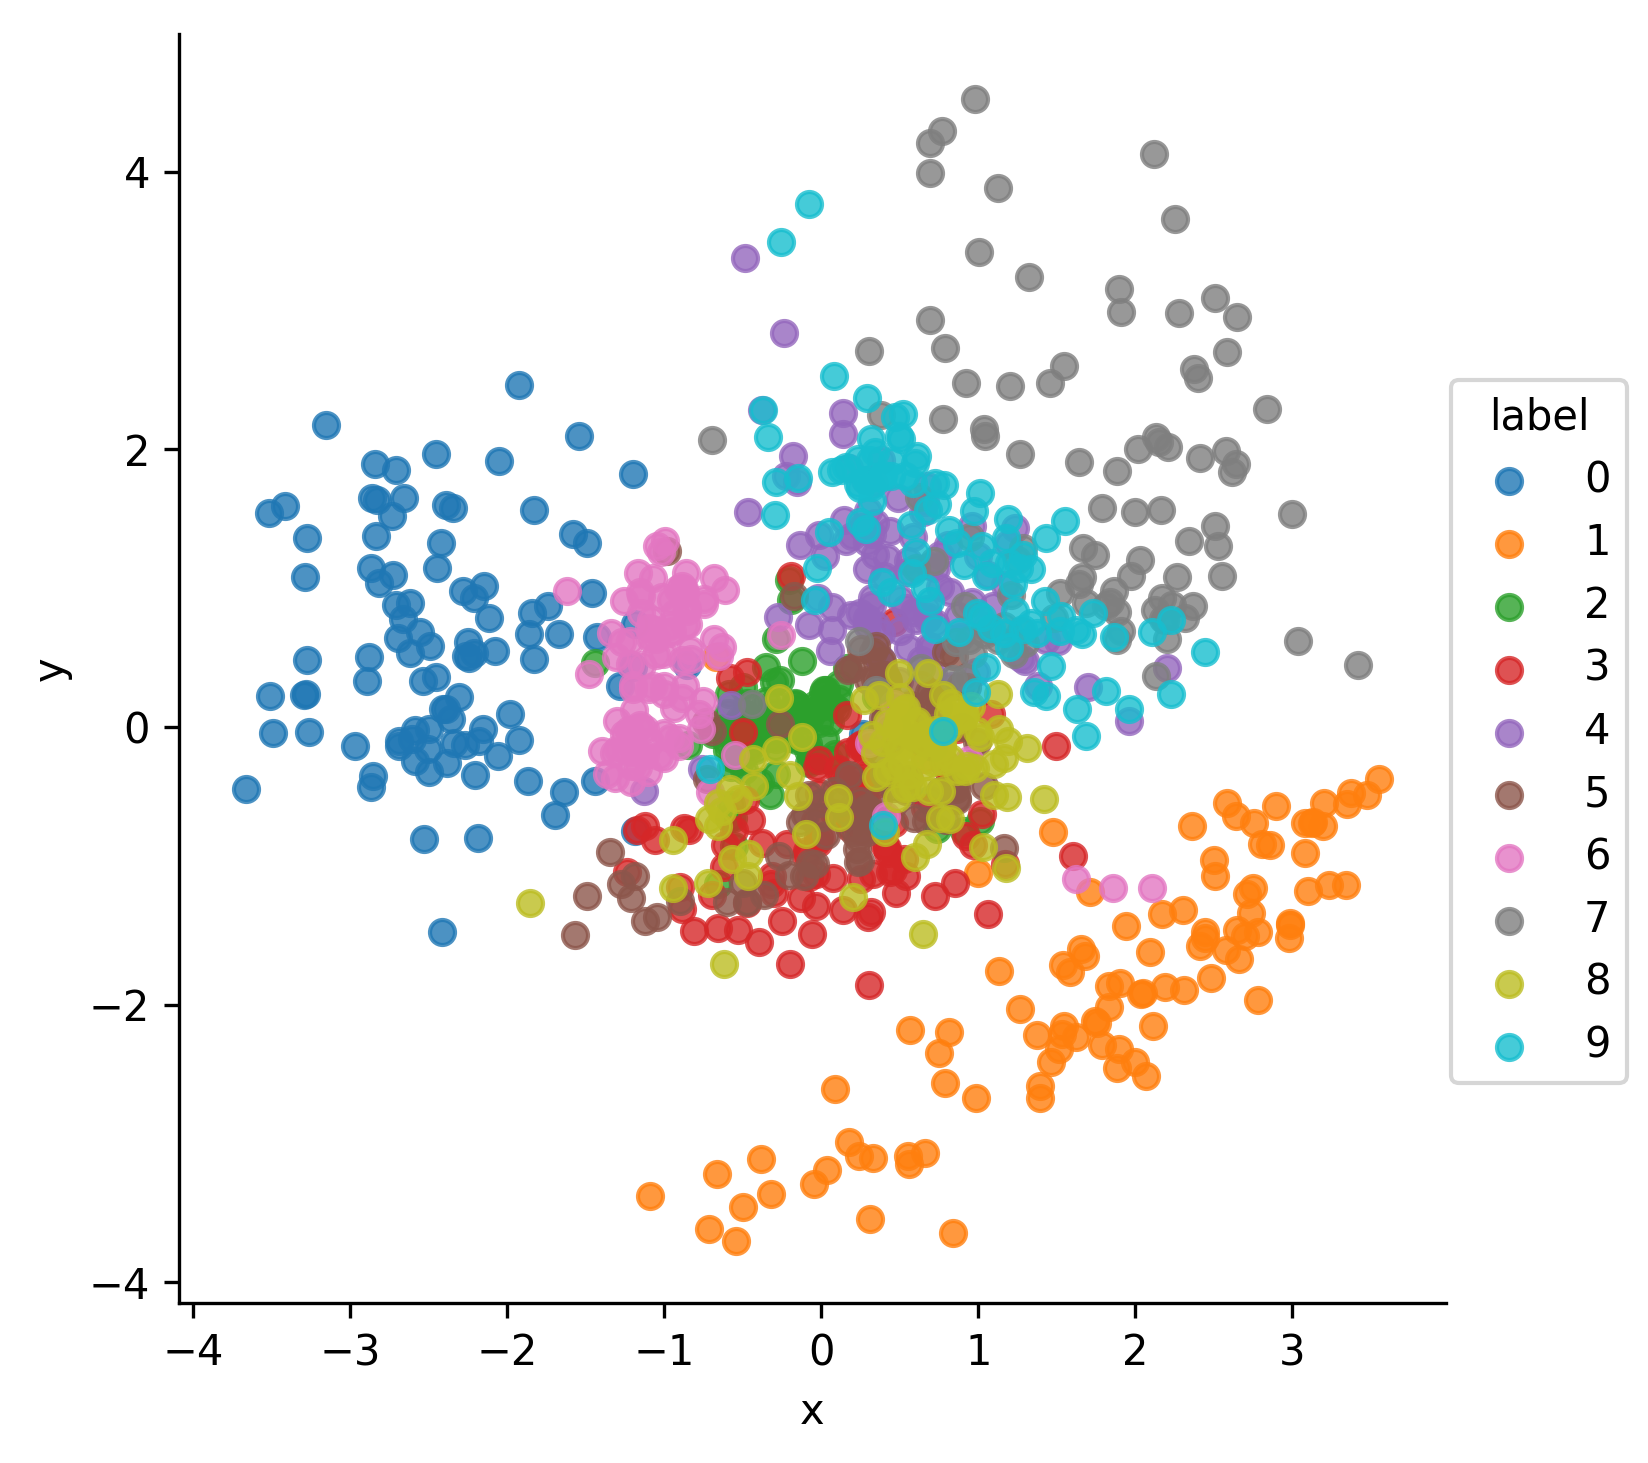
\includegraphics[width=0.45\linewidth]{figs/cvae_vae.png}
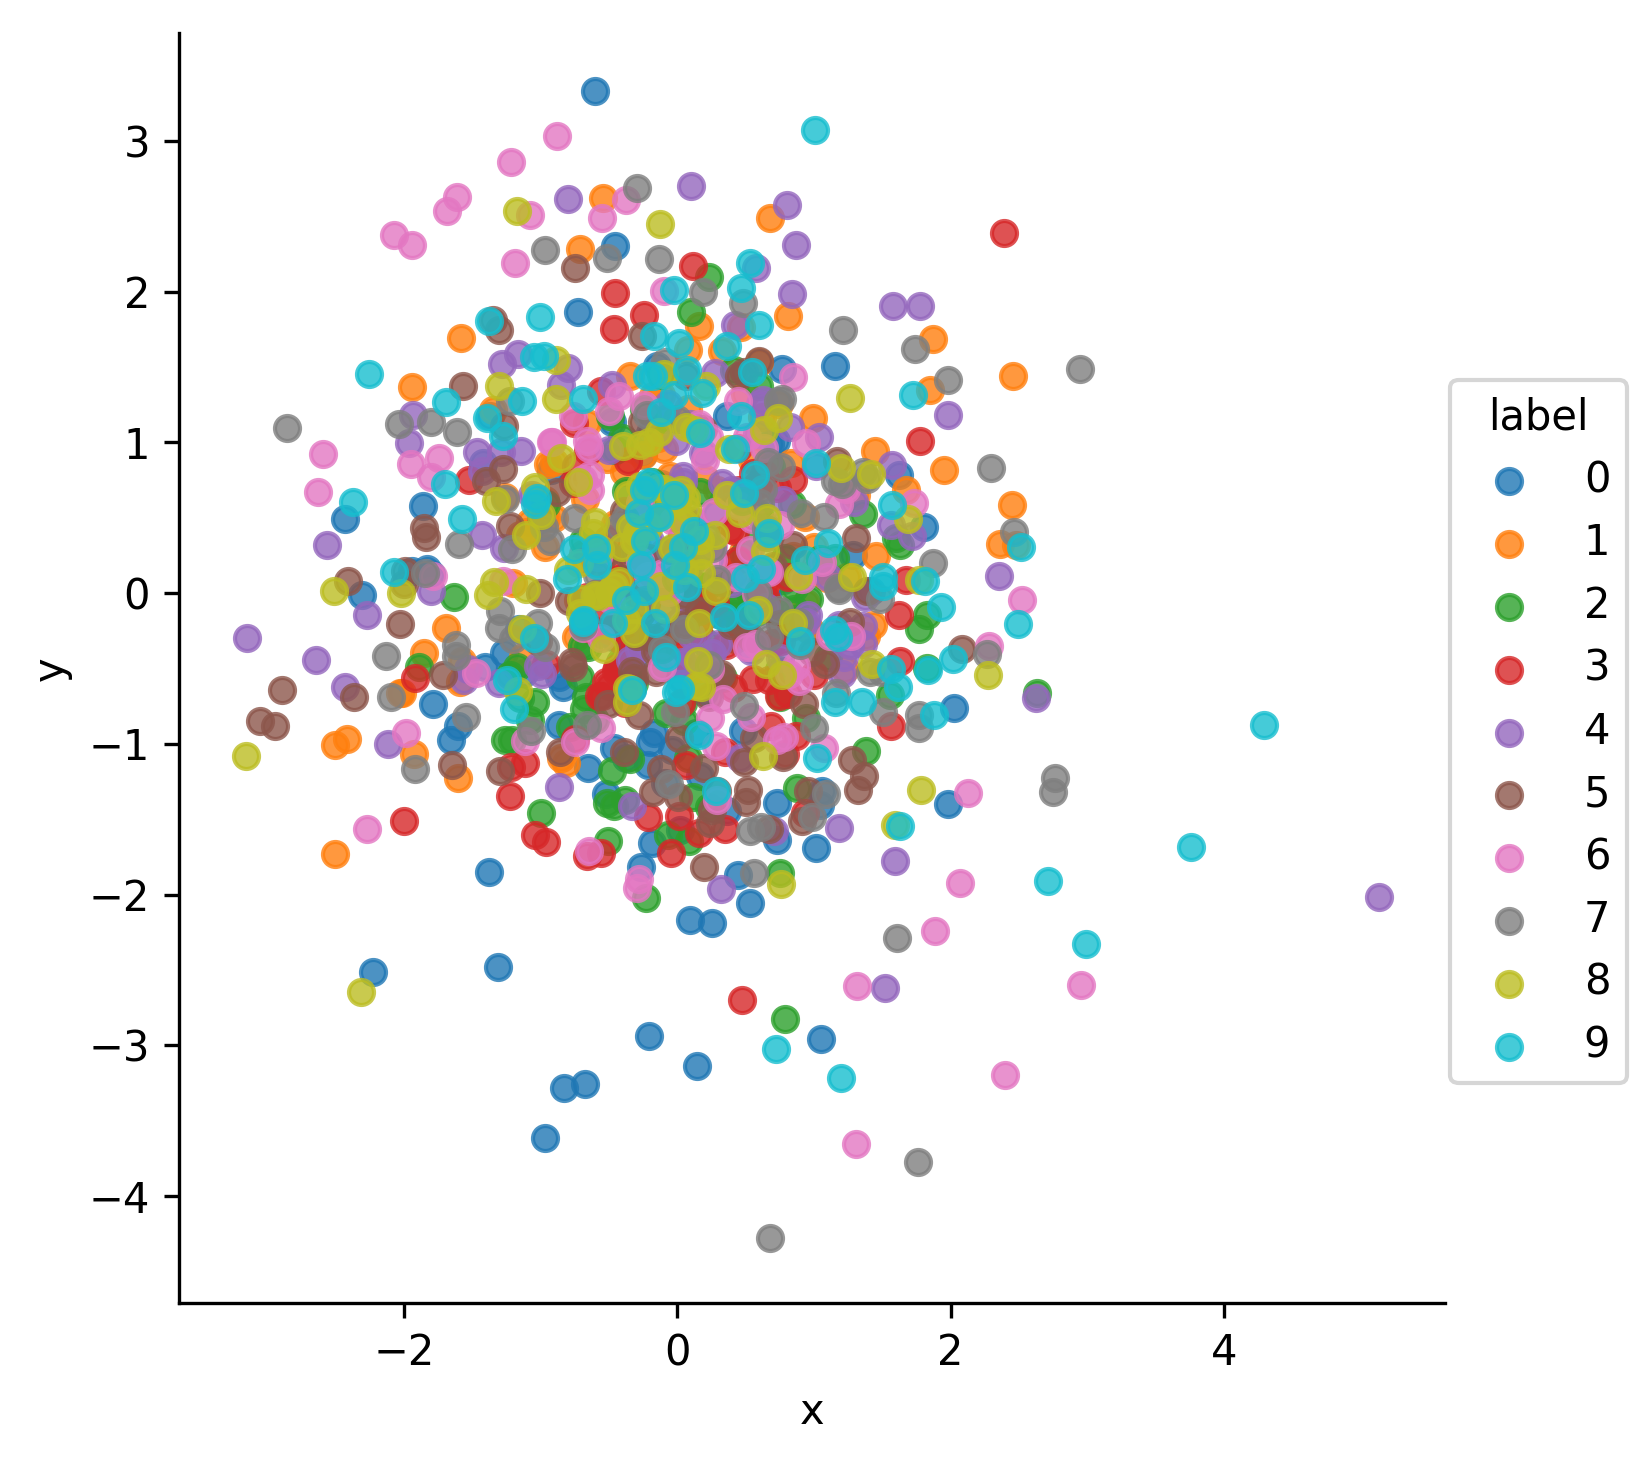
\includegraphics[width=0.45\linewidth]{figs/cvae_cvae.png}
\caption{Latent space for MNIST data: left is VAE, right is CVAE}
\end{figure}

Regular VAE has to split points belonging to different categories in the latent space, but CVAE latent space is much simpler (Gaussian) for each category, because it is conditioned on the label.

\end{frame}

\subsection{Relayr's Solution}
\begin{frame}
\frametitle{Relayr's Solution}
\begin{block}{Blog}
https://relayr.io/blog/one-model-to-rule-them-all/3/
\end{block}
\begin{figure}
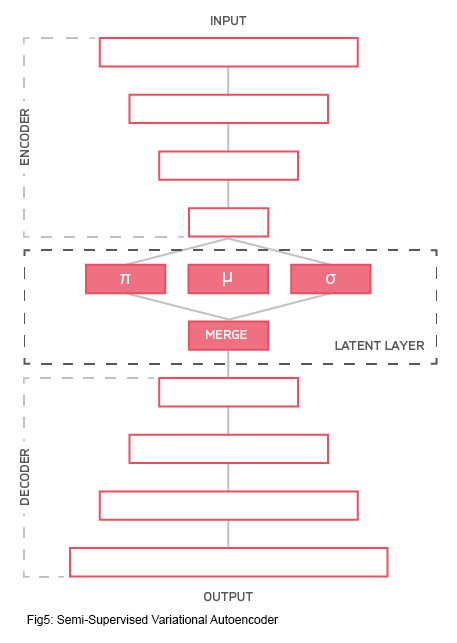
\includegraphics[width=0.4\linewidth]{figs/relayr_diagram.png}
\caption{Model Diagram}
\end{figure}
\end{frame}

\begin{frame}
\frametitle{Relayr's Solution}
\begin{block}{Loss Function}
\[
\mathcal{L} = \mathcal{L}_{\text{BCE}}(x, \hat{x}) + \mathcal{L}_{CE}(\pi, y) + KL(p(z|x)||p(z))
\]
\end{block}
where $x$ is original input; 
$\hat{x}$ is reconstructed input; 
BCE is binary cross entropy; 
CE is cross entropy;
$\pi$ is the predicted label;
$y$ is the original label;
$p(z|x)$ is the posterior distribution of latent code $z$;
$p(z)$ is prior of $z$.

As a comparison, original VAE loss is:
\[
\mathcal{L} = \mathcal{L}_{\text{BCE}}(x, \hat{x}) + KL(p(z|x)||p(z))
\]
which does not have the label term.

\end{frame}

\begin{frame}
\frametitle{Relayr's Solution}

\begin{block}{In supervised case (classification task)}
In the training, use the entire network; in the testing, cut off the decoder part.
\end{block}

\begin{block}{In anomaly detection case}
In the training, use the entire network; in the testing, cut off the $\pi$ part.
\end{block}

\begin{block}{Key}
The encoder is both a encoder and a classifier. The loss can be viewed as
$\mathcal{L} = \mathcal{L}_{CE}(\pi, y) + \mathcal{R}$, which is a regularized classifier. The entire decoder and KL is the regularizer.
\end{block}

\begin{block}{Concern}
How to merge $\pi, \mu$ and $\sigma$?
\end{block}

\end{frame}


\subsection{CVAE for Anomaly Detection and Feature Recon}
\begin{frame}
\frametitle{CVAE for Anomaly Detection and Feature Recon}
\begin{block}{Paper}
Lopez-Martin, Manuel, Belen Carro, Antonio Sanchez-Esguevillas, and Jaime Lloret. "Conditional variational autoencoder for prediction and feature recovery applied to intrusion detection in iot." Sensors 17, no. 9 (2017): 1967.
\end{block}

\begin{figure}
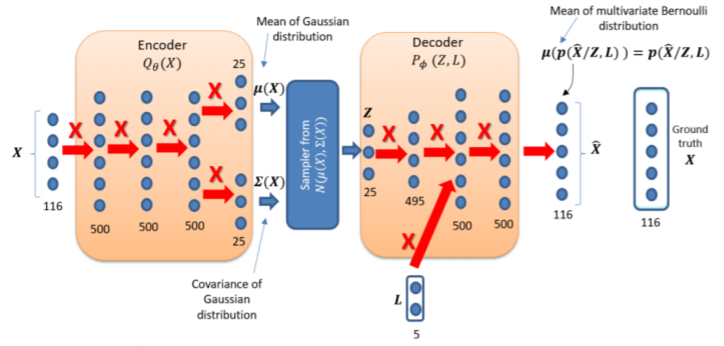
\includegraphics[width=0.8\linewidth]{figs/cvae_diagram.png}
\caption{Model Diagram}
\end{figure}

\end{frame}

\begin{frame}
\frametitle{CVAE for Anomaly Detection and Feature Recon}

\begin{block}{Classification task}
Find the label with the minimum reconstruction error.
This step requires looping all the labels, and could be time consuming.
\end{block}

\begin{block}{Feature reconstruction task}
Step 1, train the model with the data that has missing features. Step 2, given the test data with missing features, first perform the classification task and obtain the most possible label, then use the predicted label to do reconstruction (output of the decoder)
\end{block}

\begin{block}{Key}
The label is concatenated to the 3rd layer of the decoder.
\end{block}

\begin{block}{Concern}
Why concatenate the label at the 3rd layer?
\end{block}

\end{frame}


\subsection{VAE with Anomaly Prior for Anomaly Detection}
\begin{frame}
\frametitle{VAE with Anomaly Prior for Anomaly Detection}
\begin{block}{Paper}
Wang, Xuhong, et al. "Self-adversarial Variational Autoencoder with Gaussian Anomaly Prior Distribution for Anomaly Detection." arXiv (2019).
\end{block}

\begin{block}{Key}
\begin{itemize}
\setlength\itemsep{0em}
\item Propose an anomaly prior distribution
\item Propose a Transformer $T$ that maps regular latent variable to anomaly latent variable
\item Perform alternative training: train $T$ and generator $G$ in one step, train encoder $E$ in another step
\item Adv: $T$ will generate anomalous latent variables that close to the normal latent variables, and $G$ will distinguish them by different reconstruction errors.
\item Testing for anomaly is the same as other VAE based approach
\end{itemize}
\end{block}
\end{frame}

\begin{frame}
\frametitle{VAE with Anomaly Prior for Anomaly Detection}
\begin{figure}
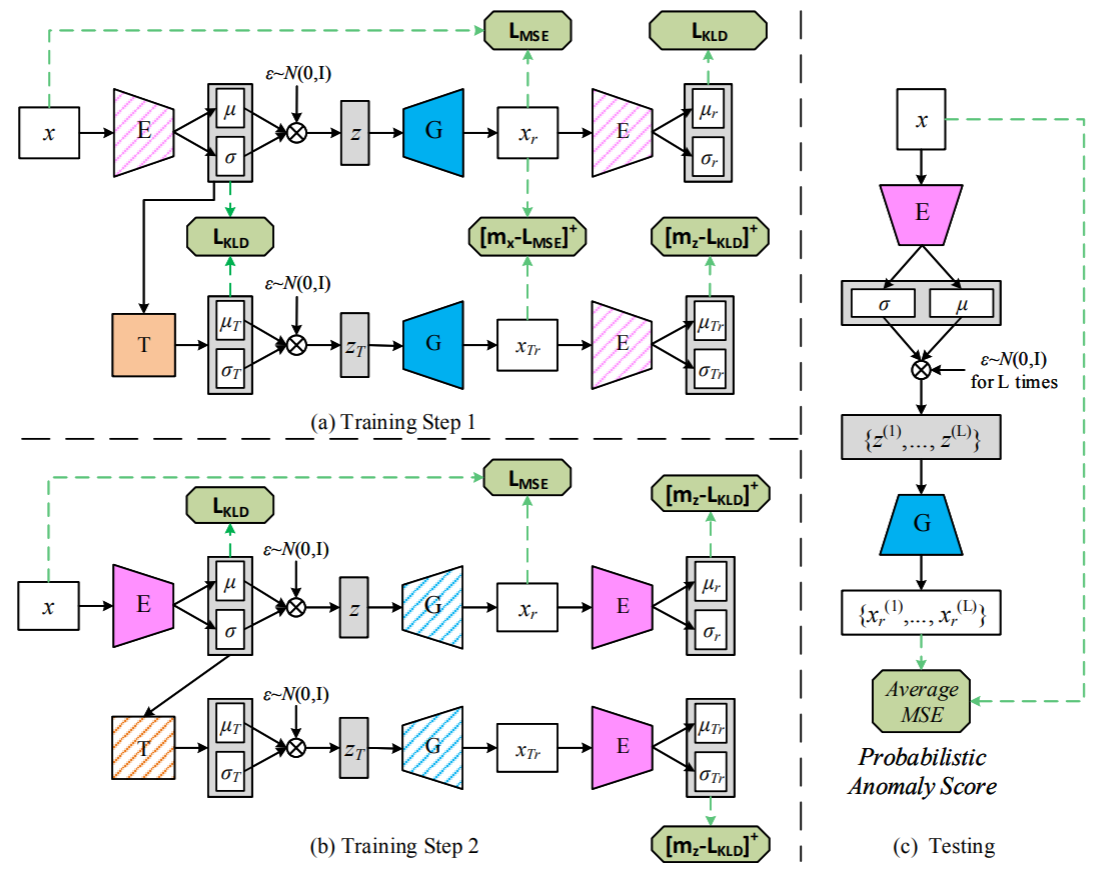
\includegraphics[width=0.8\linewidth]{figs/vae_anomaly_prior.png}
\end{figure}
\end{frame}

\begin{frame}
\frametitle{VAE with Anomaly Prior for Anomaly Detection}

\begin{block}{Train $T$ and $G$}
For $T$, minimize the difference of latent variable $z$ and $T(z)$.
\[
\mathcal{L}_T = KL(N(\mu, \sigma^2)||(N(\mu_T, \sigma_T^2))) = \log\frac{\sigma_T}{\sigma} + \frac{\sigma^2 + (\mu-\mu_T)^2}{2\sigma_T^2} - \frac{1}{2} 
\]
For $G$, two parts $\mathcal{L}_G = \mathcal{L}_{Gz} + \mathcal{L}_{GzT}$, where
\[
\mathcal{L}_{Gz} = \mathcal{L}_{MSE}(x, G(z)) + \mathcal{L}_{KLD}(E(G(z))||p(z))
\]
which is a regular VAE loss, with $p(z)$ regular prior. Also, the second part
\[
\mathcal{L}_{Gz_T} = [m_x - \mathcal{L}_{MSE}(G(z), G(z_T))]^+ + [m_z - \mathcal{L}_{KLD}(E(G(z_T))||p(z))]^+
\]
where $m_x,m_z$ are threshold params. This tries to maximize diff between $G(z)$ and $G(z_T)$, and maximize the KL of $E(G(z_T))$ and normal prior. The threshold ensure the diff is bounded.
\end{block}
\end{frame}


\begin{frame}
\frametitle{VAE with Anomaly Prior for Anomaly Detection}

\begin{block}{Train $E$}
\[
\begin{split}
\mathcal{L}_E =& \mathcal{L}_{KLD}(E(x)||p(z)) + \mathcal{L}_{MSE}(x, G(z)) \\
& + [m_z-\mathcal{L}_{KLD}(E(G(z))||p(z))]^+ + [m_z-\mathcal{L}_{KLD}(E(G(T(z)))||p(z))]^+
\end{split}
\]

The first two terms are regular VAE loss. The last two terms prevent $E$ from mapping the reconstructions to the prior distribution. 
This trains the $E$ to discriminate the training samples (normal) and their reconstruction (anomalous)
\end{block}

\begin{block}{Testing}
Testing is identical to the traditional VAE testing. Perform MC samples of encoded latent code, and set threshold on reconstruction error.
\end{block}

\end{frame}


\section{Empirical Study of Anomaly detection}
\label{sec-anomaly}
\begin{frame}
\centerline{Section~\ref{sec-anomaly}: Empirical Study of Anomaly detection}
\end{frame}

\subsection{VAE based Model}

\begin{frame}
\frametitle{VAE based Model}

\begin{block}{Methodology}
Use partial data (the data sequence exclude the last data point) to train VAE, reconstruct the full sequence. Based on the prediction error (the last data point), we set 5\% threshold on the empirical distribution. The variance in the latent space is represented by the encoder.
\end{block}

\begin{block}{Design}
\begin{itemize}
\setlength\itemsep{0em}
\item Data: Config Lab Closet Window, temperature data. Training data: 20000 points (starting from 2019-02-01 00:00:00). Testing data: 2880 points (30 days)
\item Sample rate: 15 min
\item Input: 27 points (28 exclude the last one); Output: 28 points
\item Loss: $\mathcal{L} = \alpha \mathcal{L}_{\text{recon}}(\text{27 points}) + (1-\alpha) \mathcal{L}_{\text{pred}}(\text{1 point}) + KL$
\item Encoder: 4 layers Conv + ReLU + BN, with dimension 64 to 1024 \\
\item Decoder: 4 layers, opposite to encoder. \\
\item Latent space dimension: 20
\end{itemize}
\end{block}

\end{frame}


\begin{frame}
\frametitle{VAE based Model}
\begin{figure}
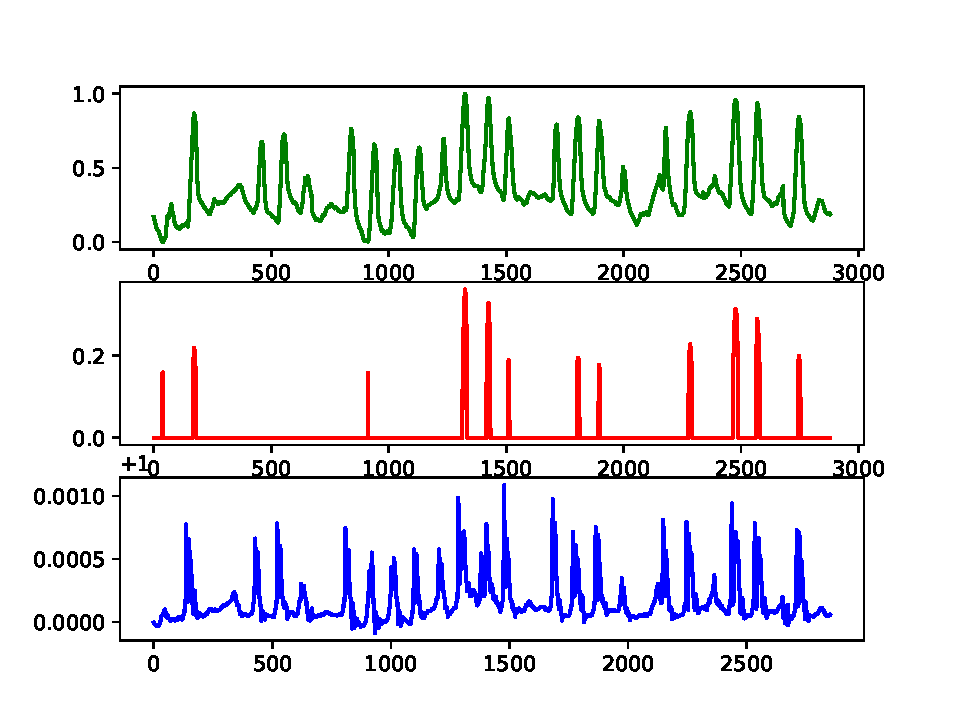
\includegraphics[width=0.8\linewidth]{figs/vae_h20_detect.pdf}
\vspace{-0.3in}
\caption{The data and prediction: from top to bottom, orignal data, detected anomaly, standard deviation of prediction}
\end{figure}
\end{frame}


\begin{frame}
\frametitle{VAE based Model}
\begin{figure}
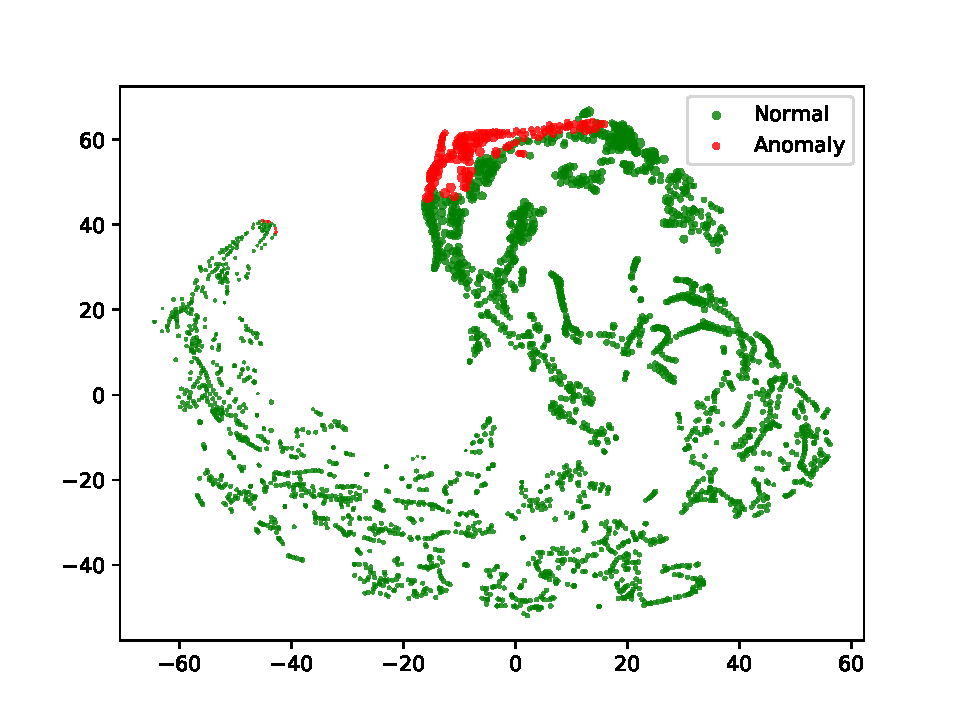
\includegraphics[width=0.45\linewidth]{figs/vae_h20_latent_anomaly.pdf}
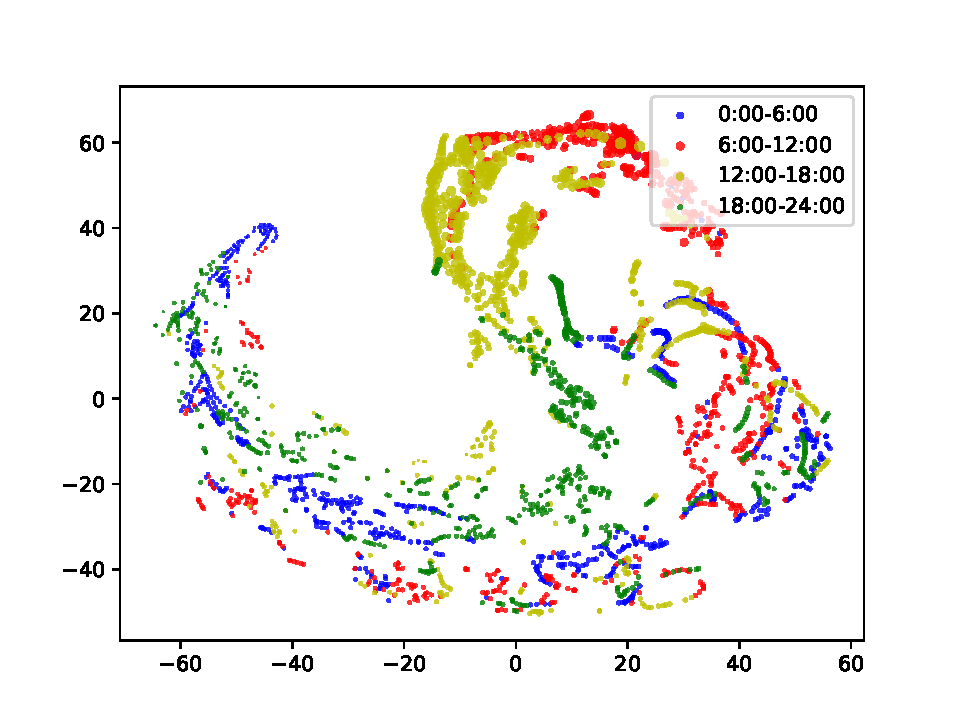
\includegraphics[width=0.45\linewidth]{figs/vae_h20_latent_time.pdf}
\vspace{-0.2in}
\caption{Latent space: left shows the anomaly data (red), right is the data for different time slots.}
\end{figure}
\vspace{-0.1in}

\begin{itemize}
\setlength\itemsep{0em}
\item The data lies in manifold, different time slots are different manifolds.
\item High prediction error corresponds to outliers in latent space.
\item The larger variance of $p(z|x)$, the larger radius of the circle in the figure.
\end{itemize}
\end{frame}


\subsection{VAE with Lower Dimensional Latent Space}

\begin{frame}
\frametitle{VAE with 5 Dimensional Latent Space}
\begin{figure}
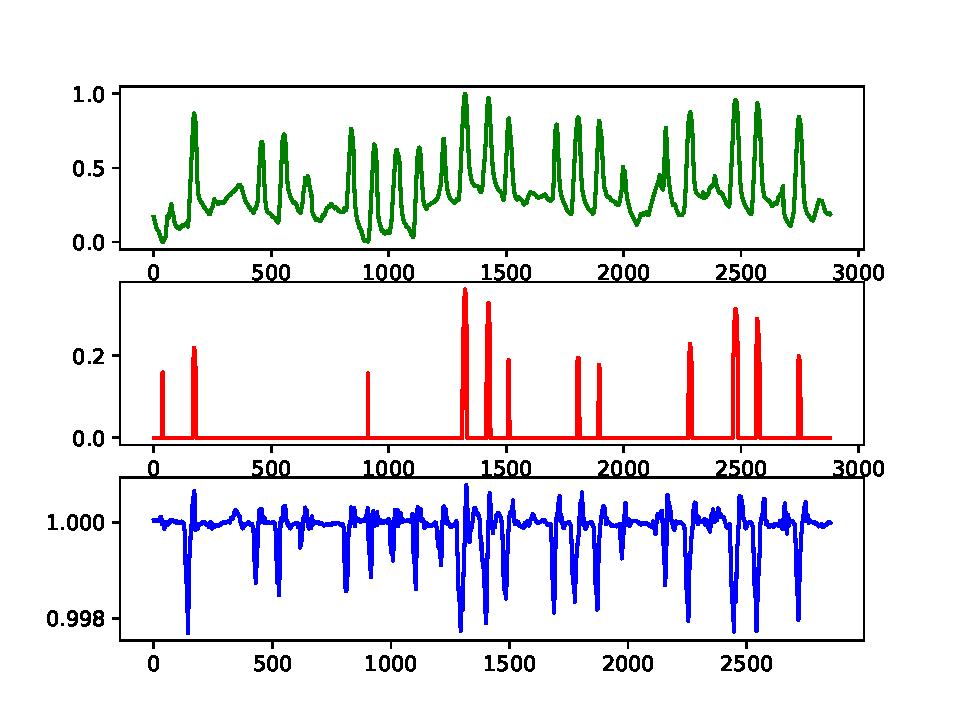
\includegraphics[width=0.8\linewidth]{figs/vae_h5_detect.pdf}
\vspace{-0.3in}
\caption{The data and prediction: from top to bottom, orignal data, detected anomaly, standard deviation of prediction}
\end{figure}
\end{frame}

\begin{frame}
\frametitle{VAE with 2 Dimensional Latent Space}
\begin{figure}
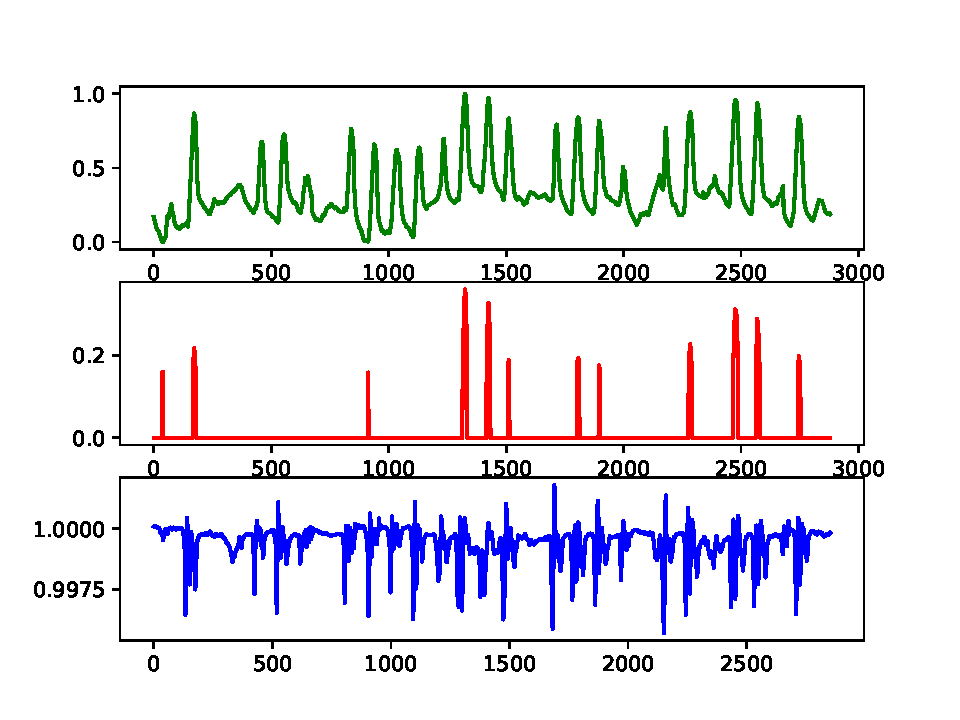
\includegraphics[width=0.8\linewidth]{figs/vae_h2_detect.pdf}
\vspace{-0.3in}
\caption{The data and prediction: from top to bottom, orignal data, detected anomaly, standard deviation of prediction}
\end{figure}
\end{frame}


\begin{frame}
\frametitle{VAE with Lower Dimensional Latent Space}
\begin{figure}
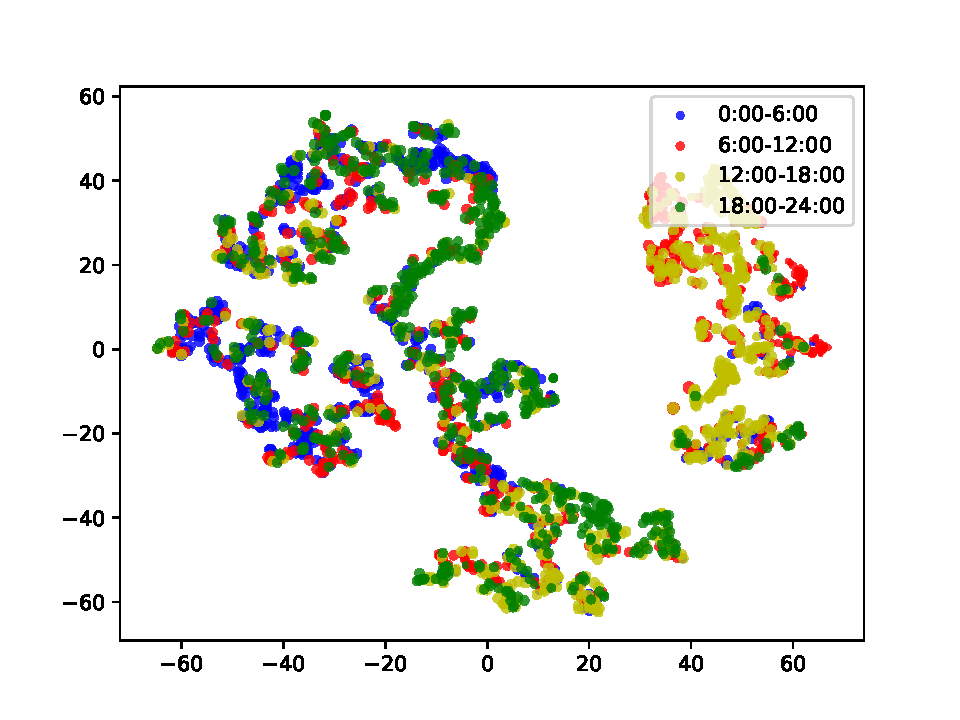
\includegraphics[width=0.32\linewidth]{figs/vae_h2_latent_time.pdf}
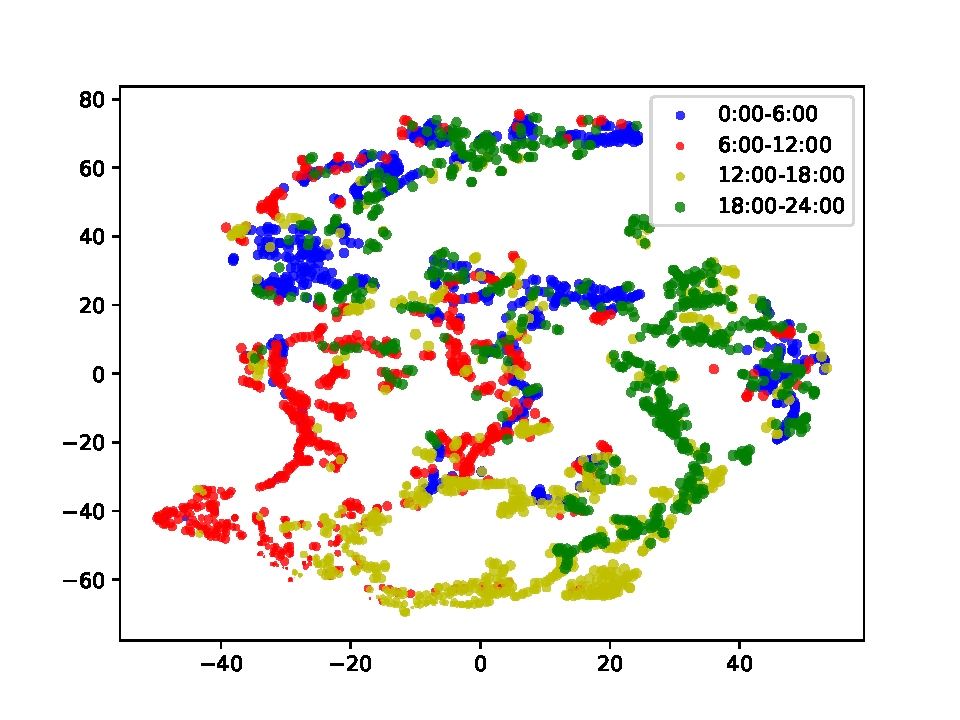
\includegraphics[width=0.32\linewidth]{figs/vae_h5_latent_time.pdf}
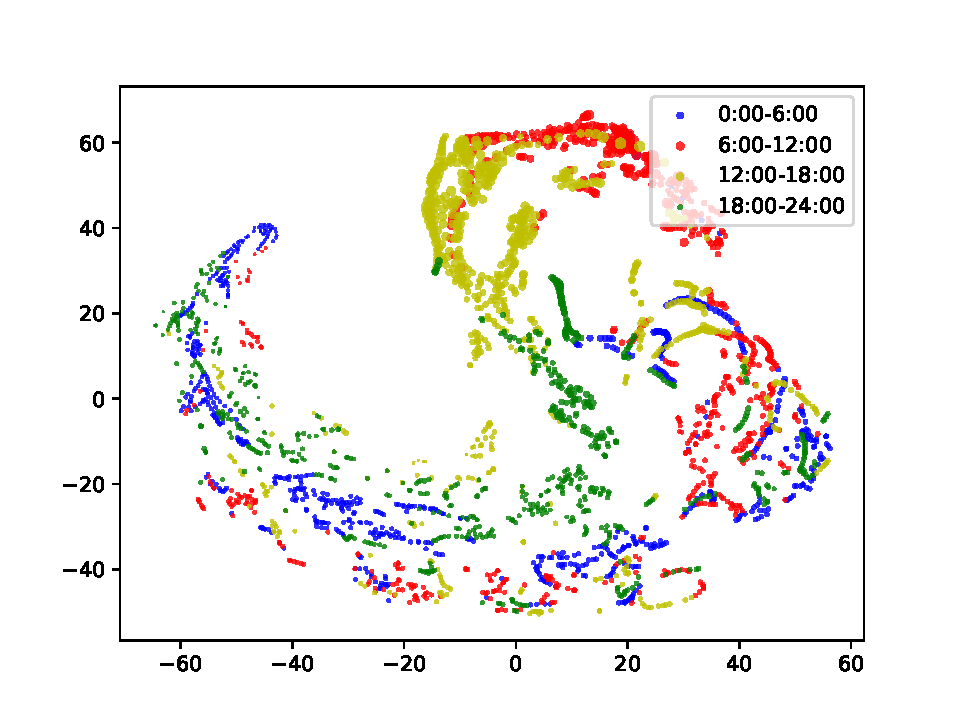
\includegraphics[width=0.32\linewidth]{figs/vae_h20_latent_time.pdf}
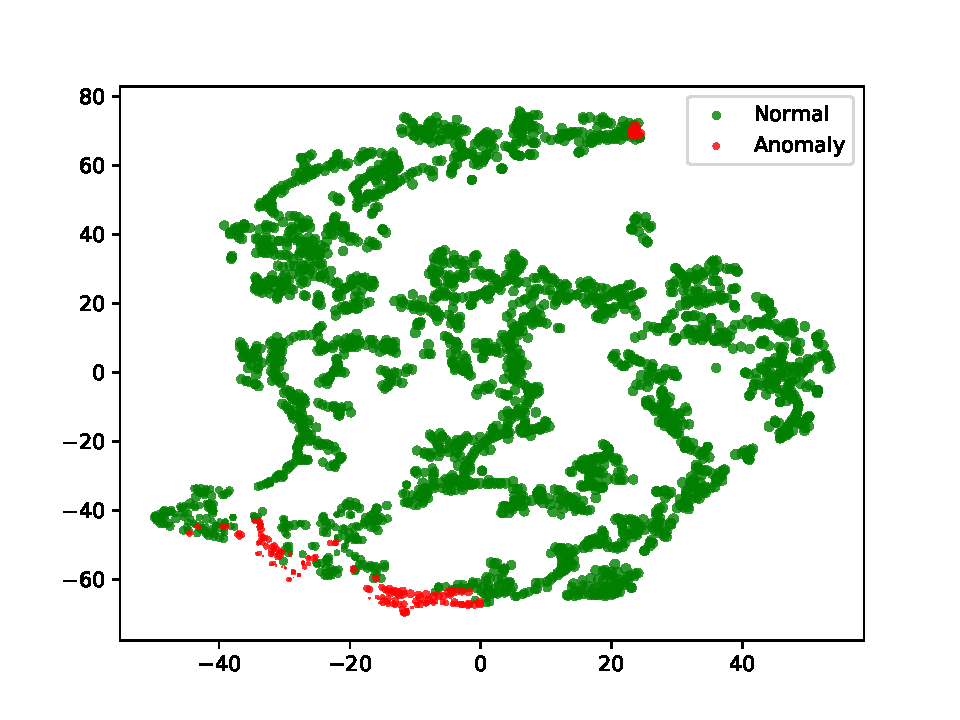
\includegraphics[width=0.32\linewidth]{figs/vae_h5_latent_anomaly.pdf}
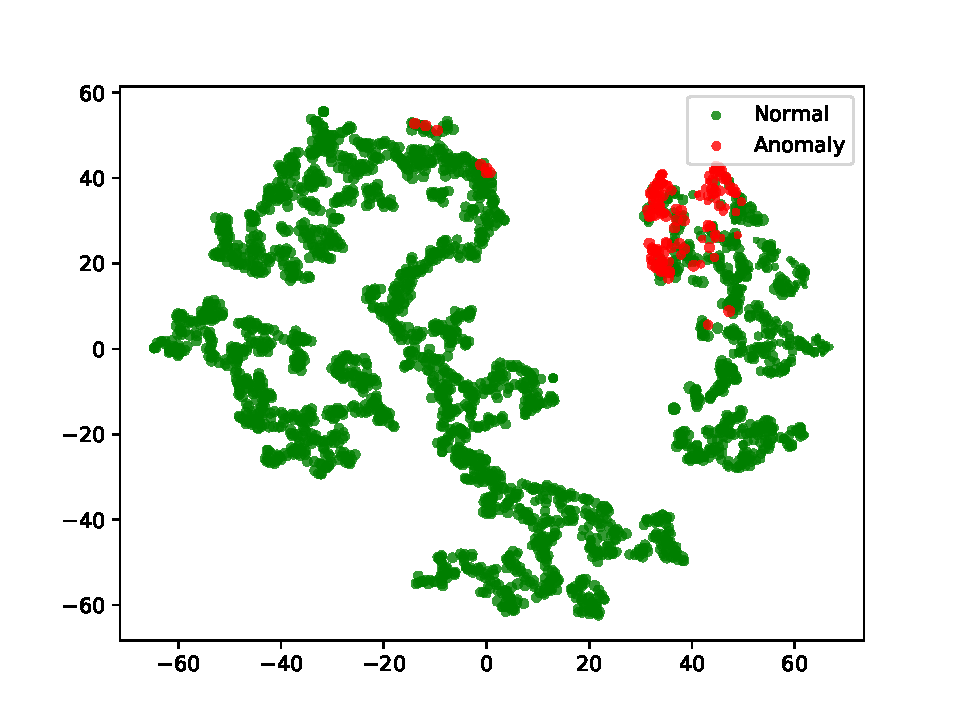
\includegraphics[width=0.32\linewidth]{figs/vae_h2_latent_anomaly.pdf}
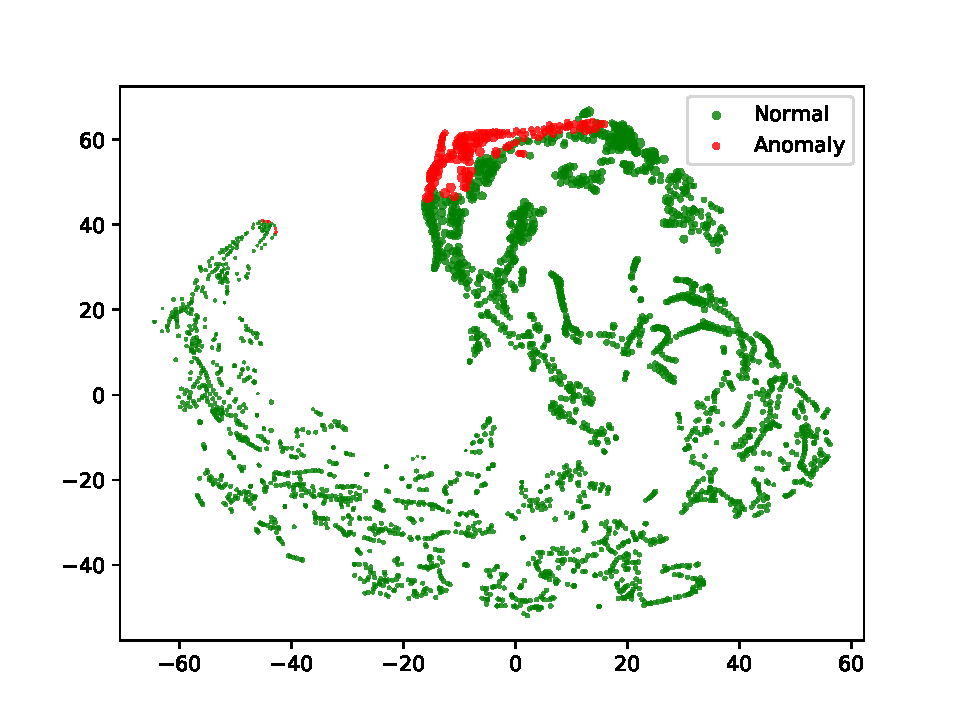
\includegraphics[width=0.32\linewidth]{figs/vae_h20_latent_anomaly.pdf}
\caption{Left to Right: 2-D, 5-D, 20-D. \ \ \ For lower latent space dimension, the manifold is less clear.}
\end{figure}
\end{frame}




\subsection{LSTM based Model}
\begin{frame}
\frametitle{LSTM based Model}

\begin{block}{Methodology}
Use sequential data train LSTM and predict the next data point. Based on the prediction error, we set 5\% threshold on the empirical distribution.
\end{block}

\begin{block}{Design}
\begin{itemize}
\setlength\itemsep{0em}
\item Sample rate: 15 min
\item Input: 27 points
\item Output: 1 point
\item Loss: MSE of the prediction 
\item State space dimension: 5
\item Model architecture 1: 2 layers LSTM + 1 layer linear (in 20, out 1)
\item Model architecture 2: 4 layers LSTM + 1 layer linear (in 20, out 1)
\item \# of forward pass: 20
\end{itemize}
\end{block}

\end{frame}

\begin{frame}
\frametitle{LSTM based Model - 2 Layers LSTM}
\begin{figure}
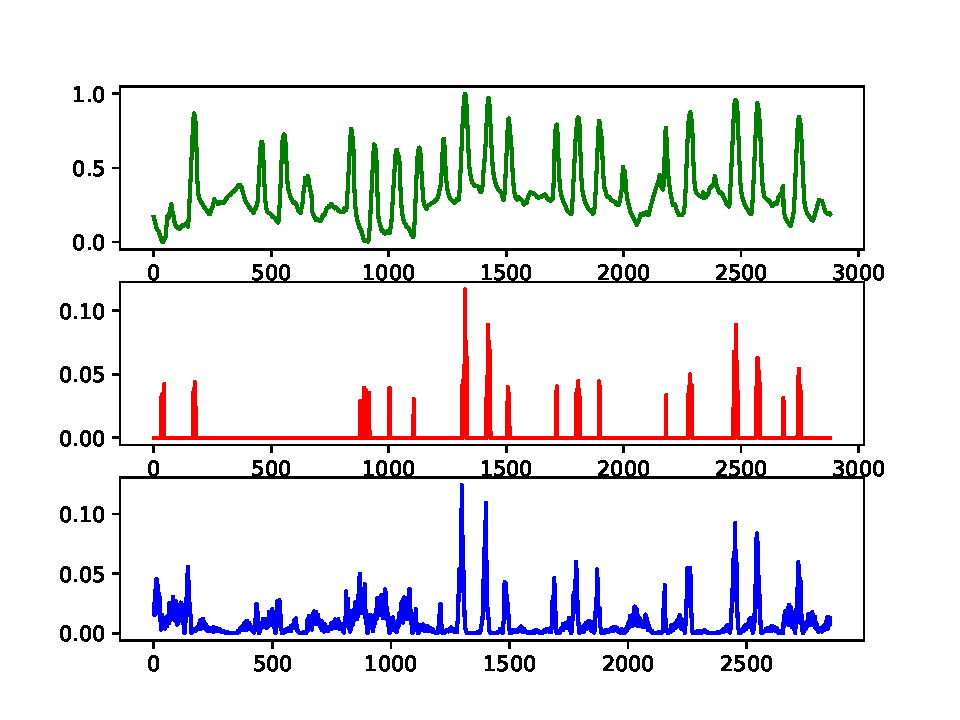
\includegraphics[width=0.8\linewidth]{figs/lstm_dropout_test_h5_detect_2layer.pdf}
\vspace{-0.3in}
\caption{The data and prediction: top is the orignal data, middle is the detected anomaly, bottom is standard deviation of prediction}
\end{figure}
\end{frame}

\begin{frame}
\frametitle{LSTM based Model - 4 Layers LSTM}
\begin{figure}
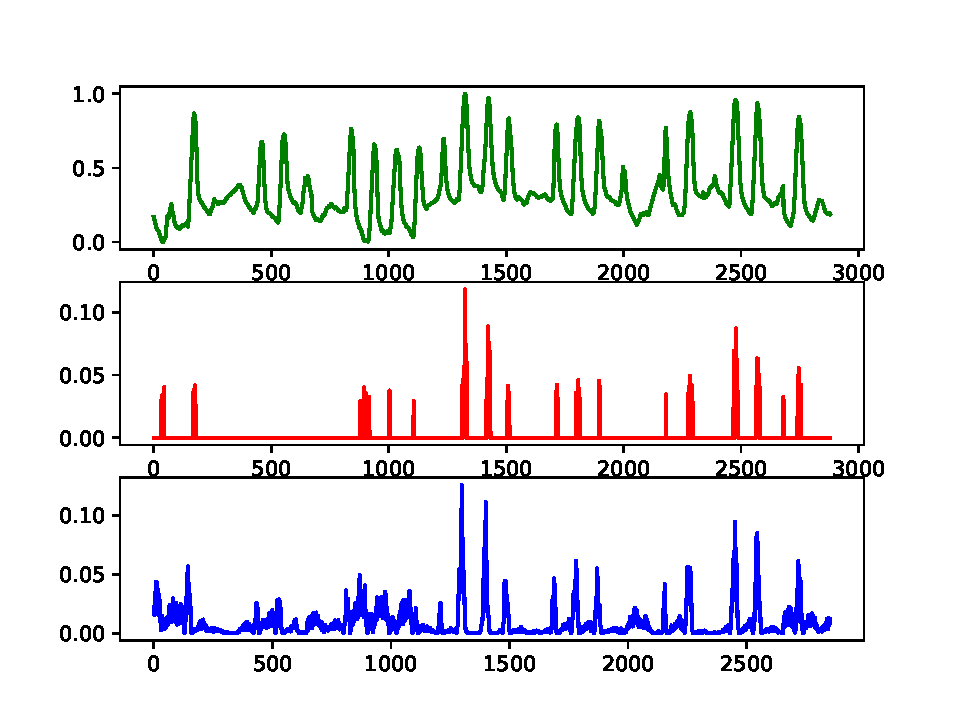
\includegraphics[width=0.8\linewidth]{figs/lstm_dropout_test_h5_detect_4layer.pdf}
\vspace{-0.3in}
\caption{The data and prediction: top is the orignal data, middle is the detected anomaly, bottom is standard deviation of prediction}
\end{figure}
\end{frame}

\subsection{LSTM Comparison}
\begin{frame}
\frametitle{LSTM with Higher Hidden State Dimension}
\begin{figure}
\vspace{-0.1in}
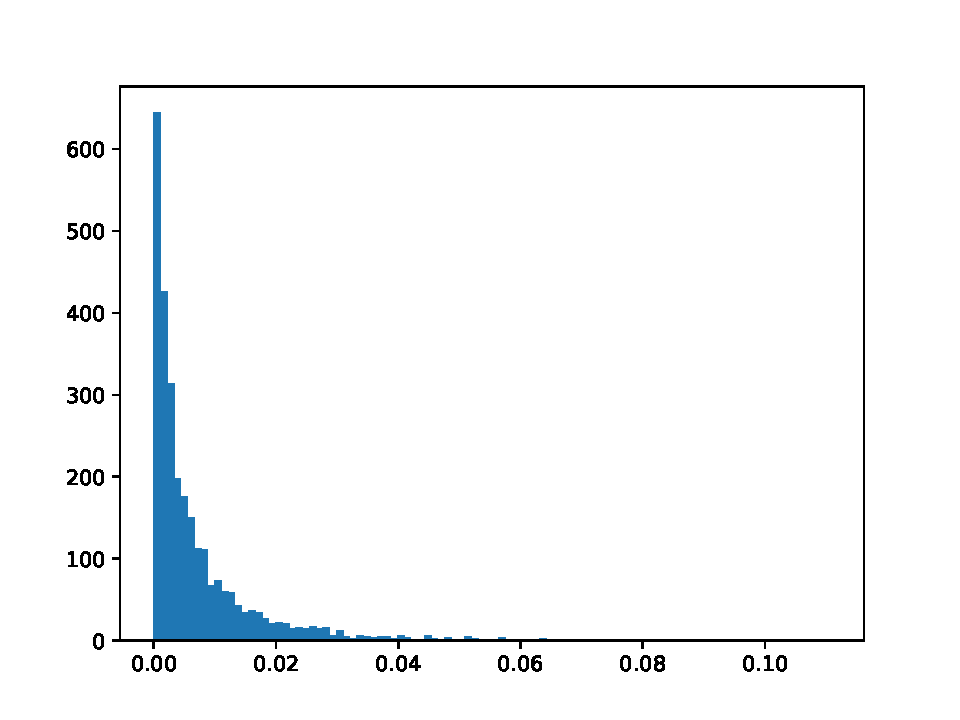
\includegraphics[width=0.4\linewidth]{figs/lstm_dropout_test_h5_pred_loss_4layer.pdf}
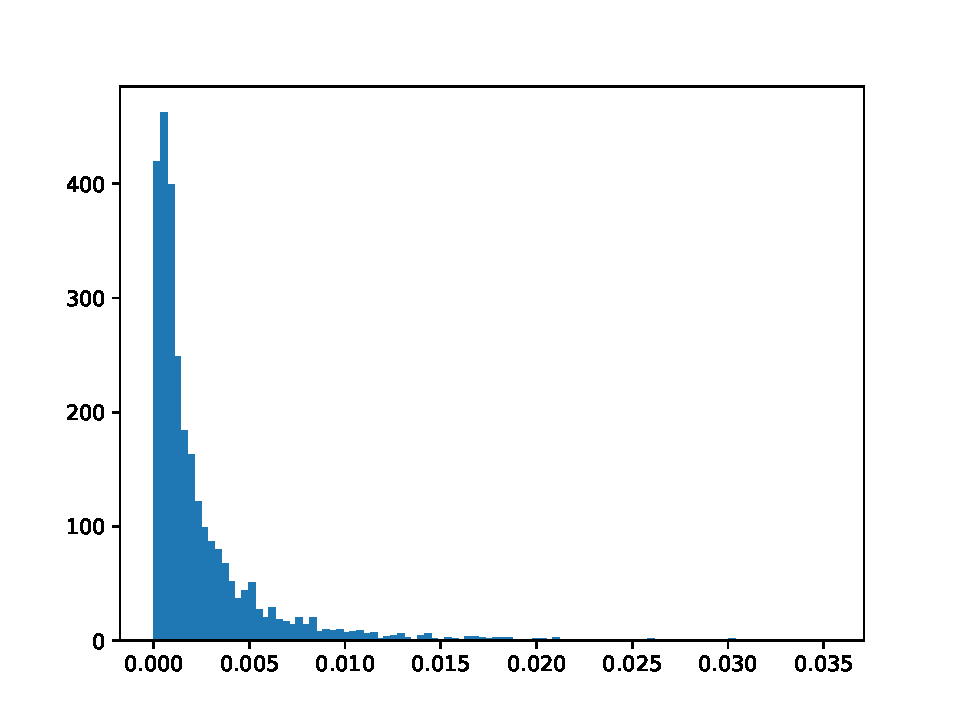
\includegraphics[width=0.4\linewidth]{figs/lstm_dropout_test_h20_pred_loss_4layer.pdf}
\vspace{-0.2in}
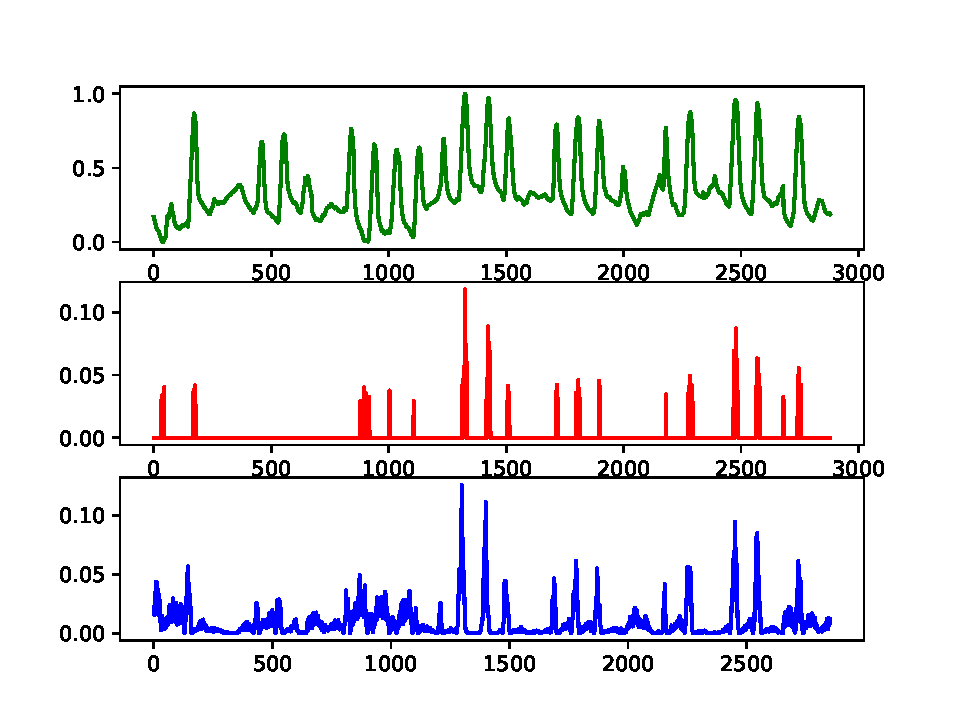
\includegraphics[width=0.4\linewidth]{figs/lstm_dropout_test_h5_detect_4layer.pdf}
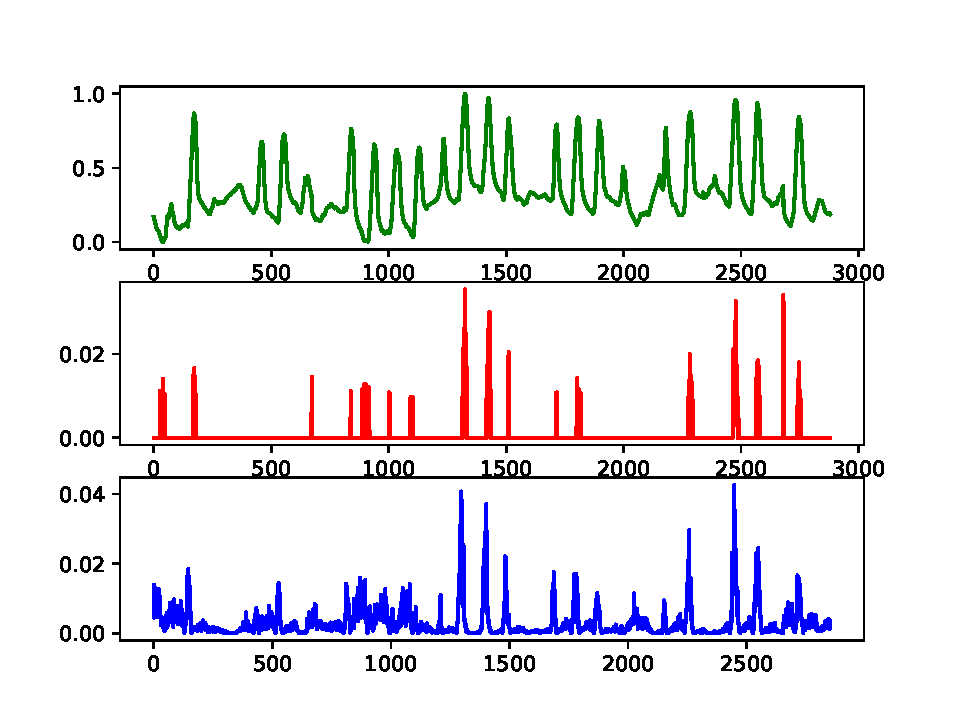
\includegraphics[width=0.4\linewidth]{figs/lstm_dropout_test_h20_detect_4layer.pdf}
\caption{Left: 5-D hidden space; Right: 20-D hidden space; Up: pred loss; Bottom: detect.}
\end{figure}
\end{frame}


\subsection{VAE and LSTM based Models Comparison}
\begin{frame}
\frametitle{Comparison}
\begin{figure}
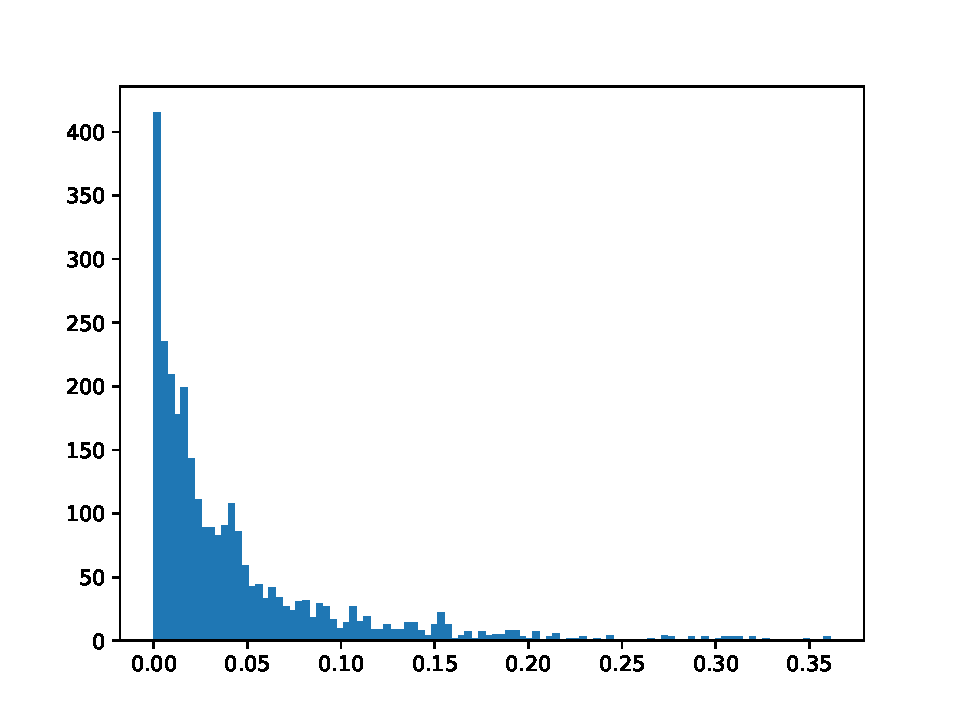
\includegraphics[width=0.32\linewidth]{figs/vae_h20_pred_loss.pdf}
%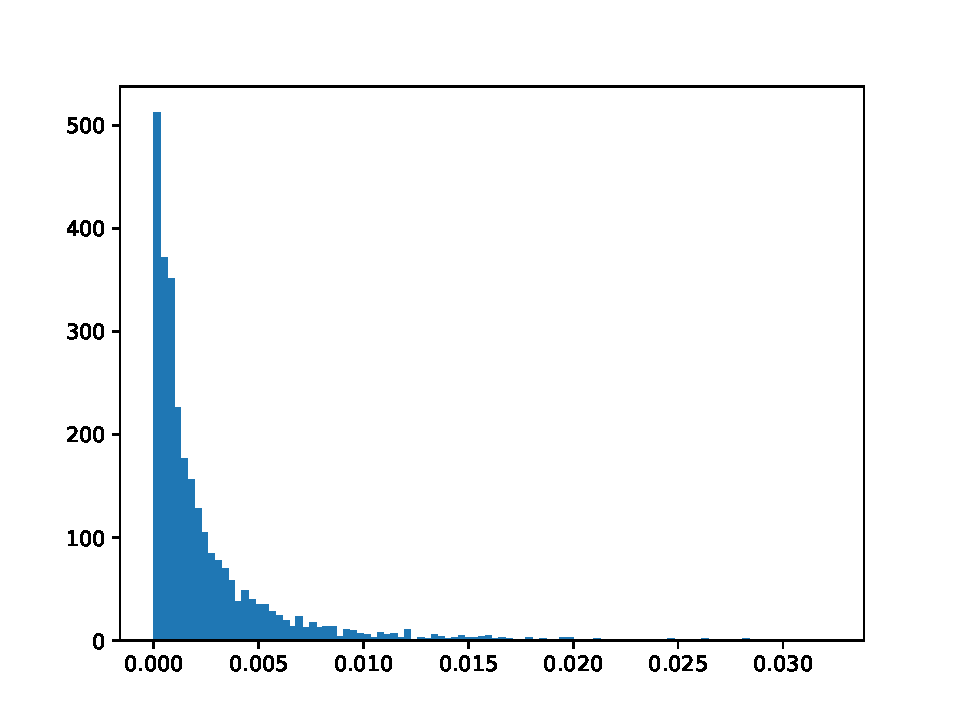
\includegraphics[width=0.24\linewidth]{figs/lstm_dropout_test_h20_pred_loss_2layer.pdf}
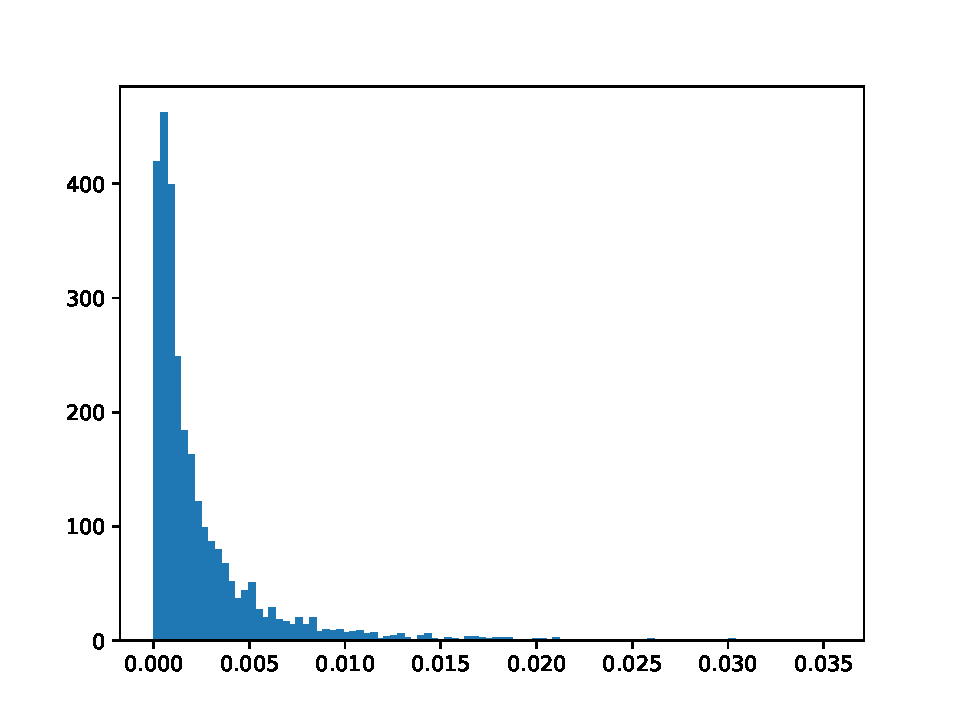
\includegraphics[width=0.32\linewidth]{figs/lstm_dropout_test_h20_pred_loss_4layer.pdf}
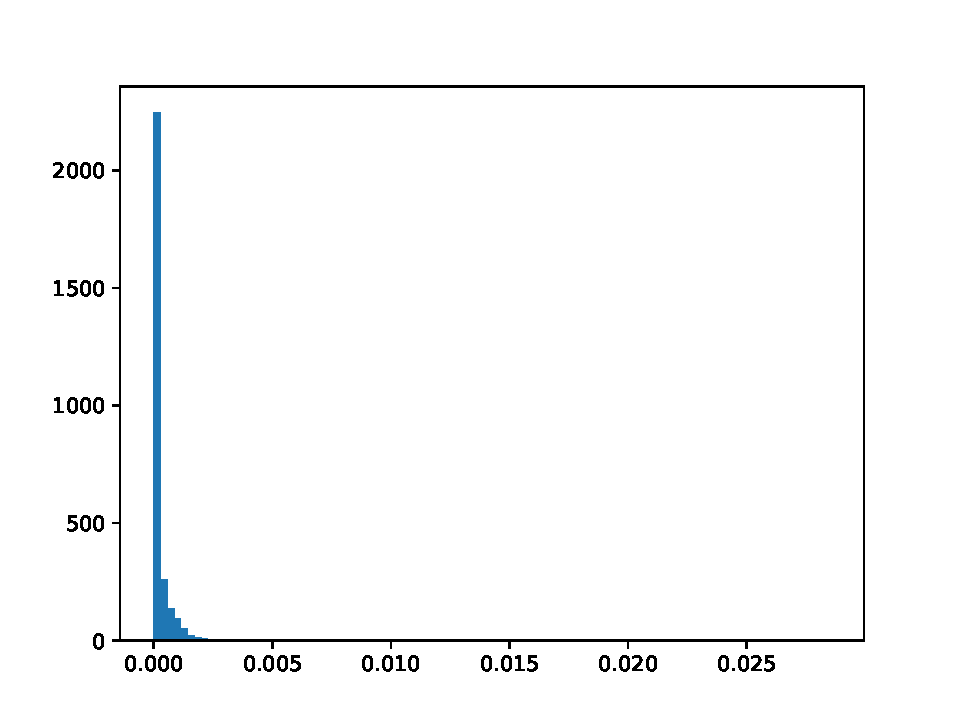
\includegraphics[width=0.32\linewidth]{figs/lstm_h20_pred_loss_4layer.pdf}
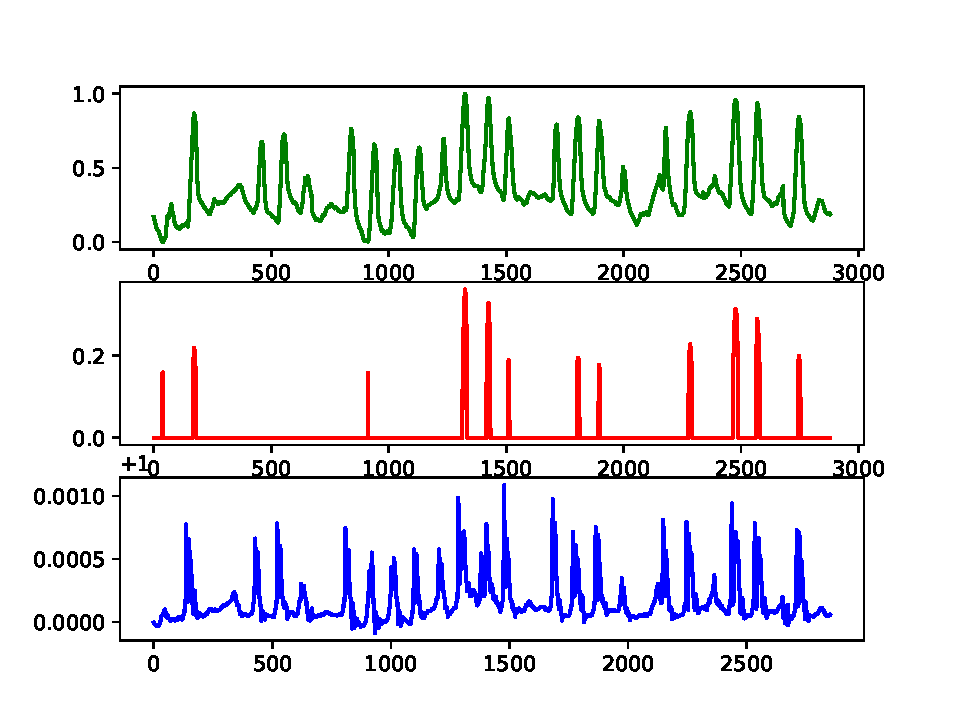
\includegraphics[width=0.32\linewidth]{figs/vae_h20_detect.pdf}
%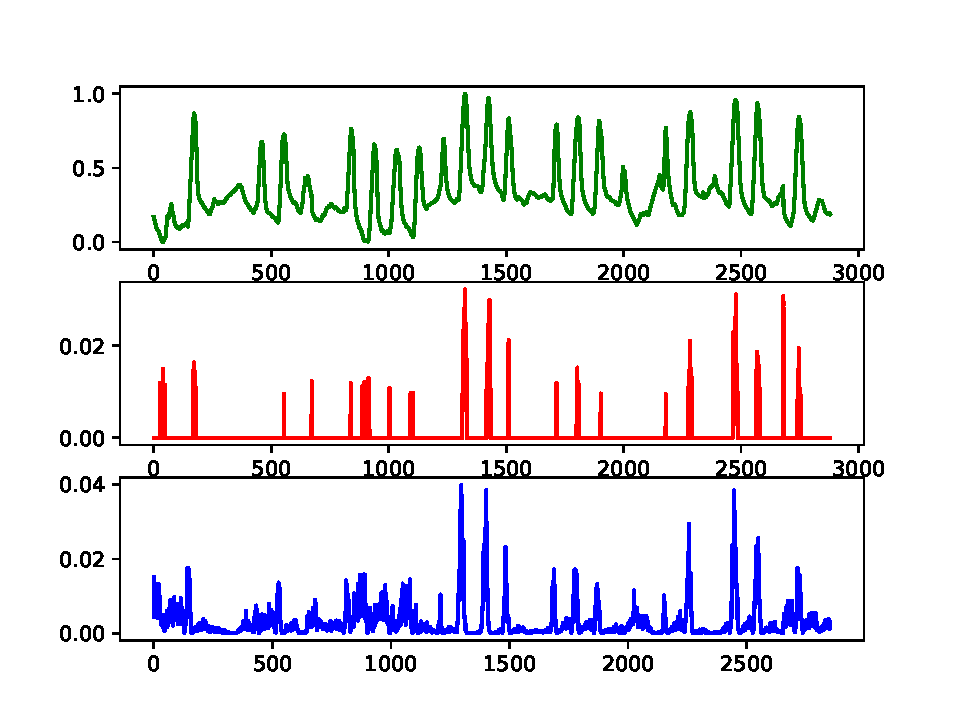
\includegraphics[width=0.32\linewidth]{figs/lstm_dropout_test_h20_detect_2layer.pdf}
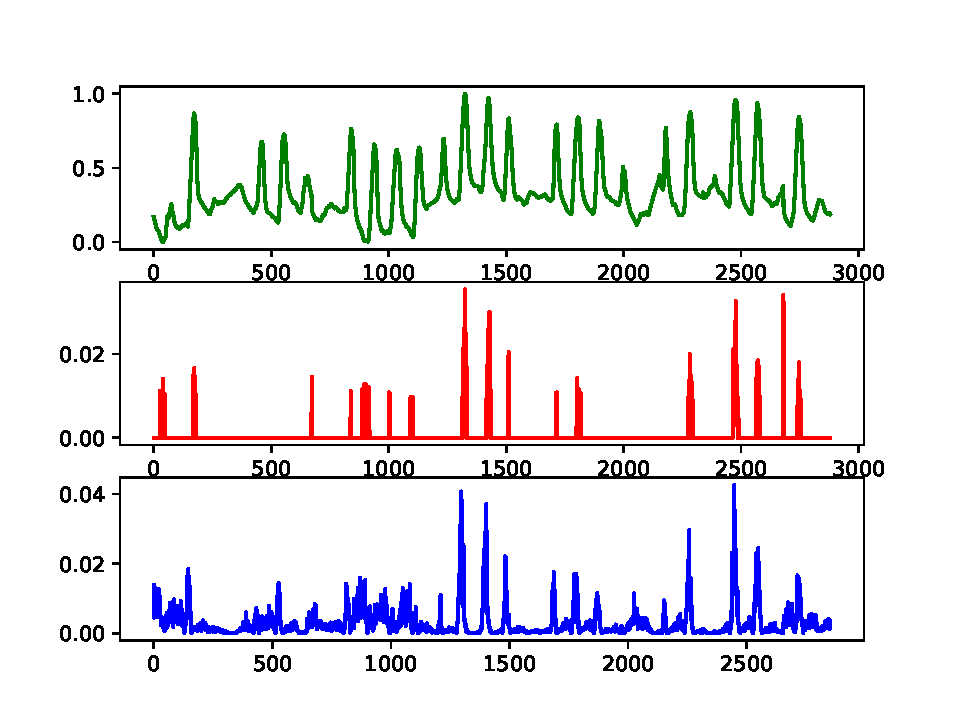
\includegraphics[width=0.32\linewidth]{figs/lstm_dropout_test_h20_detect_4layer.pdf}
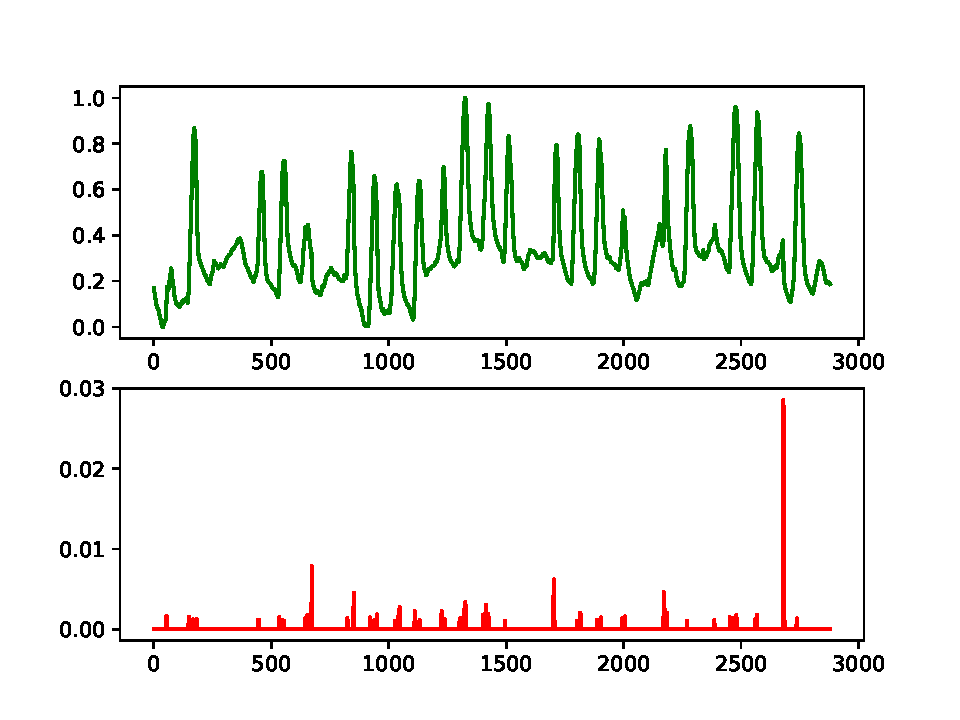
\includegraphics[width=0.32\linewidth]{figs/lstm_h20_detect_4layer.pdf}
%\vspace{-0.2in}
\caption{Row 1: prediction loss; Row 2: data and detection. \ \ \ Left to right: VAE, 4-layer LSTM with Dropout, 4-layer LSTM without Dropout}
\end{figure}
\vspace{-0.1in}


\end{frame}


\section{Adversarial Attack on Sequence Data Model}
\label{sec-advattack}
\begin{frame}
\centerline{Section~\ref{sec-advattack}: Adversarial Attack on Sequence Data Model}
\end{frame}

\subsection{Adversarial Attack on LSTM based Model}
\begin{frame}
\frametitle{Adversarial Attack on LSTM based Model}
\begin{block}{Attack Method}
The adversarial goal is to maximize the accumulated MSE of the prediction, i.e.
\[
\begin{split}
& \min_\delta \mathcal{L} = \min_\delta -\sum^N[(\mathcal{F}(x+\delta | \theta) - y)^2] \\
& \text{s.t.} \ \ \ x+\delta \in \mathcal{C} = \{x+\delta: ||x+\delta||_p \leq (1+\epsilon)||x||_p\}
\end{split}
\]
where $\mathcal{L}$ is the adversarial loss, $\mathcal{F}$ is the model, $x$ is the data, $y$ is the label, $N$ is the number of data points, $\delta$ is the modification, $\epsilon$ is the bound parameter, $\mathcal{C}$ represents the feasible set within the bound.

Using Projected Gradient Descent, we can perform the attack
\[
\hat{x} \leftarrow \text{Proj}_\mathcal{C} (x - \eta \nabla_x \mathbb{E}[\mathcal{L}])
\]
where $\text{Proj}_\mathcal{C}$ performs projection to constraint set $\mathcal{C}$.
\end{block}

\end{frame}

\begin{frame}
\frametitle{Adversarial Attack on LSTM based Model}
\begin{block}{Settings}
\begin{itemize}
\setlength\itemsep{0em}
\item $\epsilon$: we set to 0.01 and 0.05
\item $p$-norm: we use $\infty$-norm to simplify the projection
\item $\text{Proj}_{\mathcal{C}_\infty}(x)$: clamp function under $\infty$-norm
\end{itemize}
\end{block}

\begin{block}{The error amplifying ratio $\rho$}
$\rho$ is defined as the averaged prediction error after performing the attack, versus the error before attack.

\begin{table}[]
\begin{tabular}{c|ccc}
$\rho$          & 2-layer & 4-layer & 8-layer  \\
\hline
$\epsilon=0.01$ & 2.66  & 4.05  & 2.10 \\
$\epsilon=0.05$ & 21.69 & 45.86 & 12.99  \\
\end{tabular}
\end{table}
\vspace{-0.1in}
As expected, the larger $\epsilon$ the larger error. Even with 1\% modification, the error could be increased to 4 times. For 5\% modification, the error increases to 45 times.
However, for 8-layer case, it is significantly better, contrary to the common thinking.
\end{block}
\end{frame}


\subsection{Adversarial Modification Distribution}
\begin{frame}
\frametitle{Adversarial Modification Distribution}
\vspace{-0.1in}
\begin{figure}
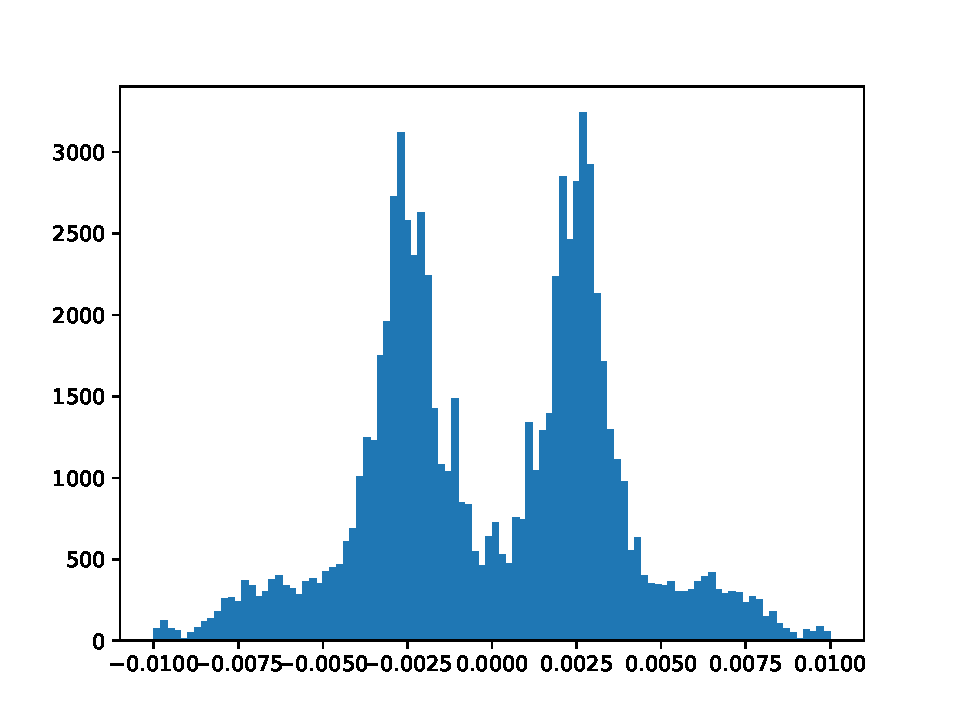
\includegraphics[width=0.32\linewidth]{figs/attack_lstm_2layer_001.pdf}
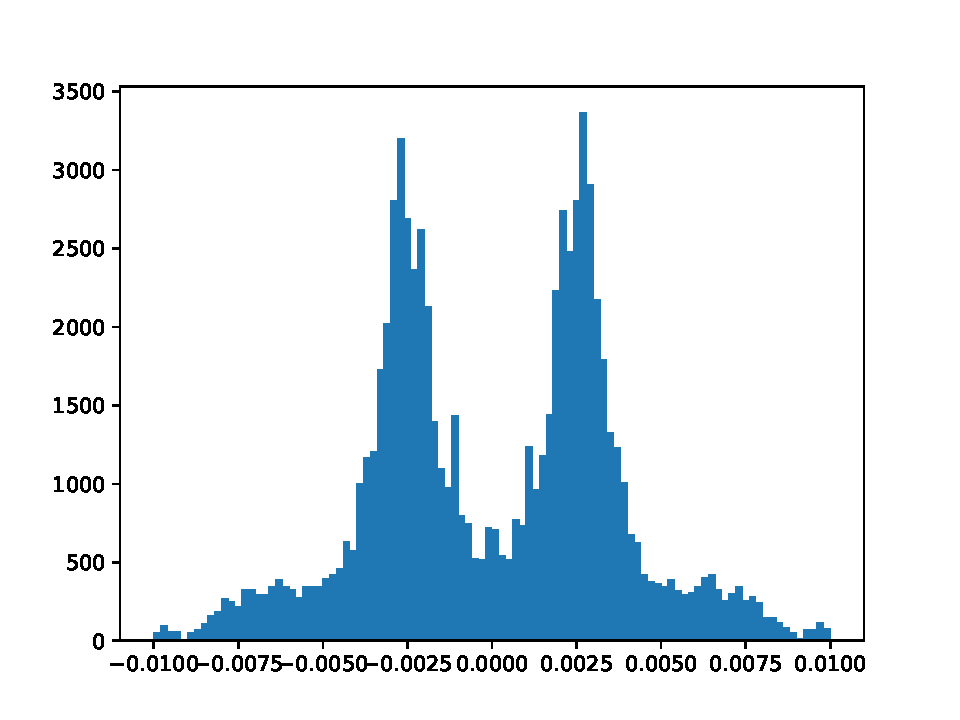
\includegraphics[width=0.32\linewidth]{figs/attack_lstm_4layer_001.pdf}
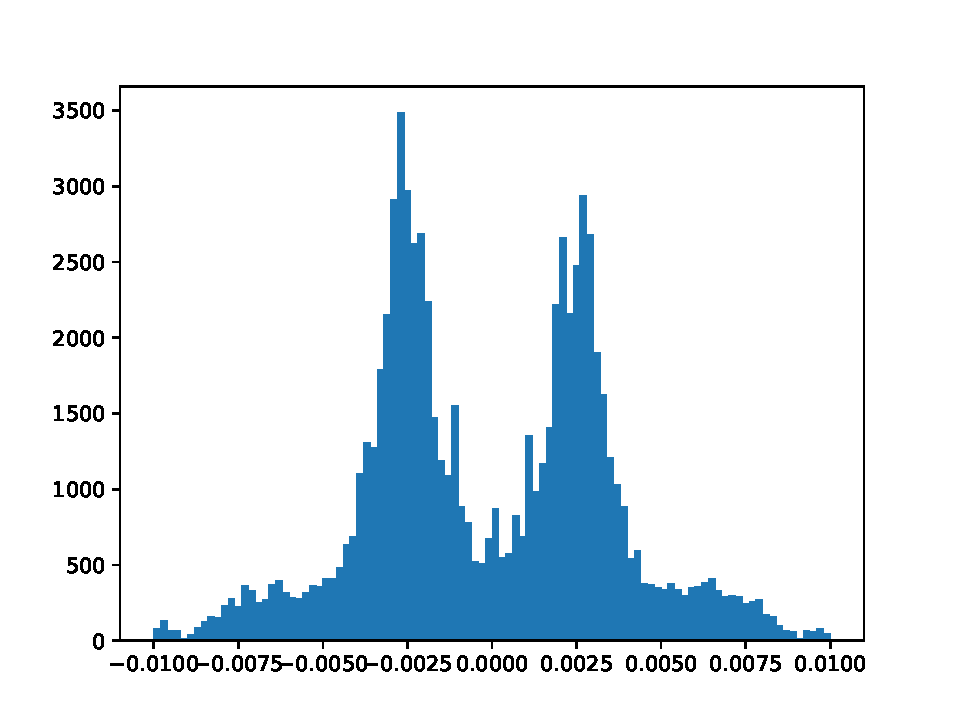
\includegraphics[width=0.32\linewidth]{figs/attack_lstm_8layer_001.pdf}
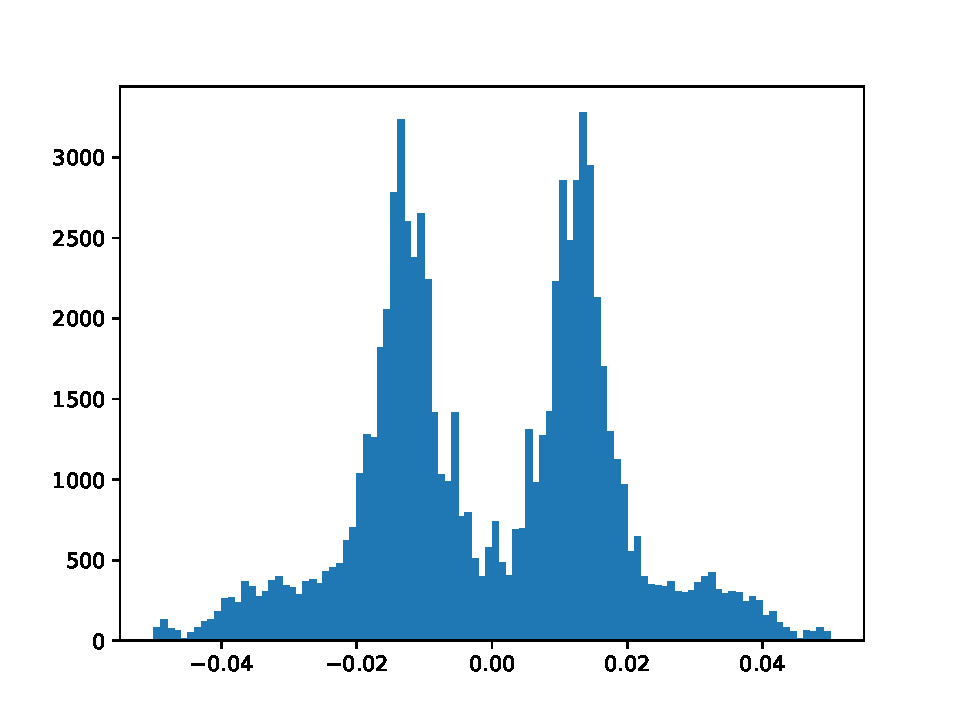
\includegraphics[width=0.32\linewidth]{figs/attack_lstm_2layer_005.pdf}
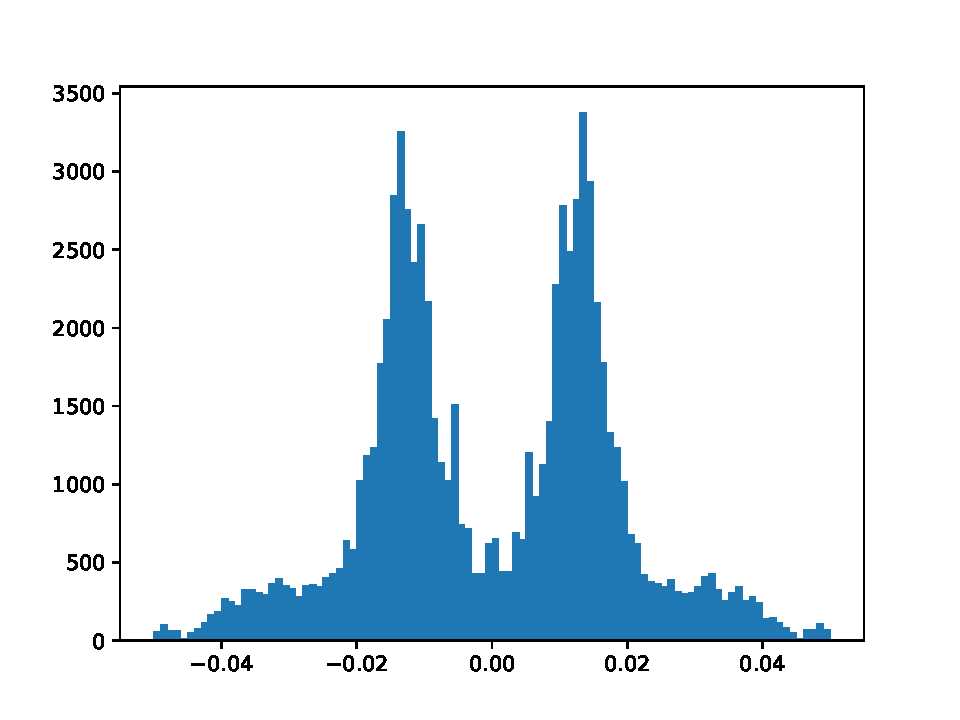
\includegraphics[width=0.32\linewidth]{figs/attack_lstm_4layer_005.pdf}
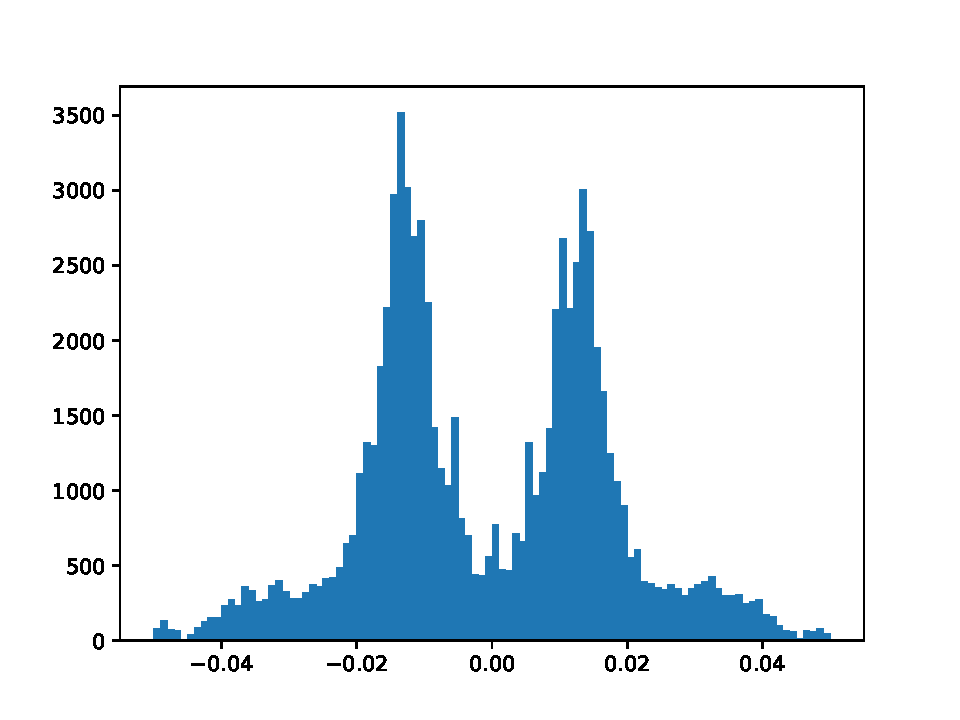
\includegraphics[width=0.32\linewidth]{figs/attack_lstm_8layer_005.pdf}
\vspace{-0.1in}
\caption{Row-1: $\epsilon=0.01$; Row-2: $\epsilon=0.05$. \ \ \ Left: 2-layer; Mid: 4-layer; Right: 8-layer. \ \ \ $|\delta|$ shows a skewed distribution. For 8-layer case, it is not symmetric.}
\end{figure}

\end{frame}

\begin{frame}
\Huge{\centerline{Thanks!}}
\end{frame}

%----------------------------------------------------------------------------------------
\end{document} 

